
\documentclass[11pt]{article}

% ---- English fonts for XeLaTeX ----
\usepackage{fontspec}
\setmainfont{Times New Roman}          % 英文正文字体
\setsansfont{Arial}                    % 英文无衬线字体
\setmonofont{Courier New}              % 英文等宽字体

% ---- ACL template ----
\usepackage[final]{acl}
\usepackage{balance}
\usepackage[final]{graphicx}
\setkeys{Gin}{draft=false}

\usepackage{dblfloatfix}

% ---- Standard packages ----
\usepackage{latexsym}
\usepackage{microtype}
\usepackage{inconsolata}  % 提升等宽字体美观度

% ---- Title box settings ----
\setlength\titlebox{3.2cm}

% ---- Optional: 英文斜体正常，中文斜体用伪斜体 ----
\XeTeXinterchartokenstate=1

% ---- Document title ----
\title{\raisebox{-0.25\height}{
\includegraphics[height=1.0cm]{figs_by_qixingyu/logo.pdf}}~Beyond OCR: A Survey of Document Intelligence\\from Structured Perception to Multimodal Question Answering}

\author{JiaShu Yang, Chi Zhang, Xingyu Qi, Ning Zhang, Jie Wu, Lingxu Chen, Jiani Guo}
\begin{document}
\maketitle
% bib, reference
% \bibliography{custom}
Documents (paper media, images, or electronic files containing textual and graphical information) are ubiquitous in daily office work, online dissemination, and governmental and enterprise workflows; automatically parsing, retrieving, and supporting decision-making based on their content constitutes a core requirement of Document Intelligence. In real-world settings, many documents are first converted into images via scanning or photographing; consequently, document processing typically starts from visual inputs: on the one hand, the system must accurately localize layout elements such as text blocks, tables, figures, and headings, and perform text detection and recognition; on the other hand, it must conduct higher-level semantic understanding and reasoning based on structured inputs to answer queries, extract key information, and generate verifiable results. With advances in deep learning and large language models, the research focus has gradually expanded from ``character-level recognition'' to ``document-level understanding and question answering'' across regions, pages, and modalities, and the field has correspondingly developed evaluation benchmarks that emphasize end-to-end capability and robustness.

Following this evolution, this paper organizes the survey in the order of ``perception first, then reasoning, and finally end-to-end unified modeling,'' and aligns evaluation suites with methodological lineages. Part I (Document Layout Analysis and OCR) focuses on layout parsing starting from page geometry, including detection/segmentation-based layout element recognition, layout-aware models that incorporate layout information into pretrained representation learning, and robustness and cross-domain generalization under real-world document distributions; it further reviews key technical points of OCR from traditional pipelines to deep learning and lightweight deployment, emphasizing error propagation and engineering constraints when OCR serves as the ``entry point'' for downstream understanding tasks. Part II (Document Understanding and Question Answering) systematically summarizes three mainstream scenarios built on structured inputs: structure-aware representations for tables, modular/executable reasoning and verifiable question answering; retrieval-augmented generation (RAG) and reasoning-driven retrieval for long texts; and multimodal pretraining and instruction alignment for visually rich documents, along with the evolution toward OCR-free modeling and multi-page, long-context understanding. Finally, we summarize the datasets and benchmarks associated with these two stages, covering task settings from single-page to multi-page documents and from closed sets to real-world enterprise documents, providing reproducible baselines for comparison and a systematic research roadmap for future studies.
% supplementary materials

\begin{figure*}[t]
\centering
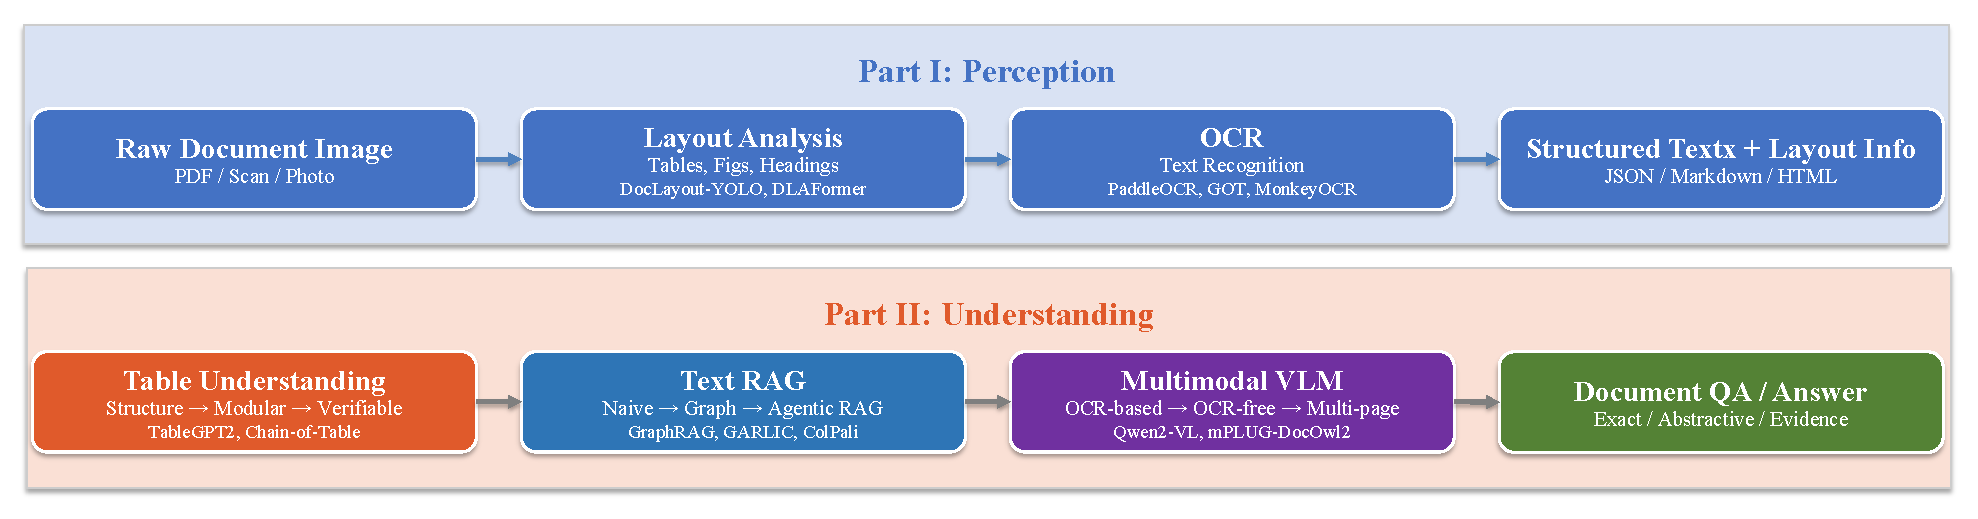
\includegraphics[
    width=0.95\textwidth,
    trim=0cm 0cm 0cm 0cm,
    clip
]{figs_by_qixingyu/fig01.pdf}
\caption{Overview of the Document Intelligence pipeline: Part~I (Perception) covers layout analysis and OCR, producing structured text and layout; Part~II (Understanding) includes three parallel branches---table understanding, text RAG, and multimodal VLM---each converging on the final Document QA output.}
\label{fig:pipeline_overview}
\end{figure*}

\section{Document Layout Analysis and OCR}

\subsection{Summary of Document Layout Analysis}
\subsubsection{Geometric Structure Detection and Analysis}

This line of work treats document layout as a purely visual or geometric structure, with the core objective of locating and classifying elements such as text blocks, images, and tables on a page. These methods output structured layout segmentation results that serve as fundamental inputs for subsequent document understanding tasks. Early work, such as The Document Spectrum for Page Layout Analysis \cite{ogorman1993documentspectrum}, characterized the overall page structure from a signal processing perspective. Document layout analysis for semantic information extraction \cite{ferrara2017documentlayoutsemantic} and Visual Detection with Context for Document Layout Analysis \cite{soto2019visual} gradually combined layout analysis with information extraction requirements and contextual modeling; the latter introduced object detection frameworks like Faster R-CNN and explicitly utilized contextual information to improve detection robustness in complex layouts. With the development of deep learning, a large body of research began adopting CNN- or Transformer-based detection models for layout analysis. For instance, Document Layout Analysis with an Enhanced Object Detector \cite{minouei2021enhancedobjectdetector} used convolutional neural networks to estimate document structure boundaries, whereas Transformer-Based Approach for Document Layout Understanding \cite{yang2022transformerlayout} introduced global self-attention for document layout understanding. Document Layout Analysis Via Positional Encoding \cite{zhou2022positionalencodinglayout} employed positional encoding to alleviate the insufficient modeling of long-range spatial relationships by traditional detectors in complex layouts. VSR: A Unified Framework for Document Layout Analysis Combining Vision, Semantics and Relations \cite{zhang2021vsr} enhanced interaction modeling between layout elements by fusing vision, semantics, and relation modules. a Graphical Approach to Document Layout Analysis \cite{wang2023graphicallayout} utilized graph structures to establish global relationships between PDF elements and improve efficiency. Advanced Layout Analysis Models for Docling \cite{livathinos2025docling} evaluated the practicality of various object detection architectures, such as RT-DETR and DFINE, in industrial-grade systems. Addressing issues of generalization and adaptation to real-world scenarios, In-domain versus Out-of-domain Transfer Learning for Document Layout Analysis \cite{li2024indomain} systematically analyzed cross-domain performance degradation, while LD-DOC proposed a lightweight domain-adaptive layout analysis method to enhance cross-domain generalization \cite{gao2024lddoc}. Regarding detection framework design, recent methods have continuously improved model unification and efficiency. a Hybrid Approach for Document Layout Analysis in Document Images \cite{hybrid_dla_2024} enhanced the multi-scale and multi-category recognition capabilities of Transformer-based detectors through a hybrid matching mechanism. DocLayout-YOLO \cite{doclayout_yolo_2024} balanced speed and accuracy by combining high-quality synthetic data with global-to-local perception modules. PP-DocLayout \cite{pp_doclayout_2025} proposed a unified detection model to support large-scale data construction, while DLAFormer \cite{dlaformer_2024} and Doc-DINO \cite{doc_dino_2024} further explored end-to-end Transformer architectures to unify the modeling of detection, classification, and logical structural relationships.

\subsubsection{Layout-Aware Representation Learning}

In this stage, layout information is explicitly integrated into the model’s representation learning process and jointly modeled with text content, enabling the model to capture implicit spatial structures and semantic relationships at the representational level. Since LayoutLM \cite{xu2019layoutlm} first introduced the joint modeling of text content and 2D positional information into the Transformer pre-training framework, document layout understanding transitioned from pure visual parsing to a representation learning paradigm. This work allowed the model to jointly learn text and layout during pre-training by modeling token coordinate embeddings alongside text embeddings. However, relying solely on coordinate embeddings and text masking tasks made it difficult to fully characterize complex spatial relationships. Position Masking \cite{saha2021position} proposed masking both text and positional embeddings during pre-training, forcing the model to explicitly predict spatial positions and thereby strengthening its ability to model positional semantics.

In the multimodal direction, LAMPRET \cite{wu2021lampret} further introduced visual features into layout-aware pre-training, aligning text, layout, and visual information through cross-modal contrastive learning. Addressing the issue that traditional methods implicitly rely on language-specific features, LiLT \cite{wang2022lilt} proposed a language-independent Layout Transformer that modeled spatial relationships between tokens through a layout-only self-attention mechanism, enhancing robustness in cross-lingual and low-resource scenarios. XYLayoutLM \cite{gu2022xylayoutlm} focused on OCR ordering noise and the insufficient modeling of reading orders, introducing the Augmented XY Cut algorithm to generate more reasonable token sequences combined with dilated conditional position encodings to improve stability in complex layouts. Regarding the expressive power of spatial relationships, ERNIE-Layout \cite{peng2022ernie_layout} explicitly modeled richer spatial and structural relationships on a page through layout-knowledge-enhanced pre-training tasks. Beyond Layout Embedding \cite{zhu2023beyond_layout} approached the problem from the attention mechanism level, introducing Gaussian-bias-based layout attention, allowing the model to dynamically adjust attention distributions based on the relative distance and orientation between entities.

Furthermore, LayoutMask \cite{tu2023layoutmask} strengthened the semantic interaction between text and layout during pre-training by designing differentiated masking strategies for different layout units. Beyond pre-training objectives and attention mechanisms, the layout representation format itself has continued to evolve. Multi-scale Cell-based Layout Representation \cite{shi2023multiscale_cell} proposed a cell-level layout representation based on row and column indices, fusing word-level and cell-level spatial information through a multi-scale design to make layout expression closer to the document’s hierarchical logical structure. In recent years, research has begun to explicitly model layout structures in relational forms. Modeling Layout Reading Order as Ordering Relations \cite{zhang2024reading_order_relations} elevated reading order from a linear sequence to directed ordering relations, injecting these relations as enhancement signals into the layout-aware model’s attention. Based on this, a Graph-Augmented Multi-Stage Transformer Model \cite{arshad2025graph_augmented} further introduced graph neural networks and a multi-stage Transformer architecture to progressively refine fine-grained structural representations by explicitly modeling the spatial and semantic relationships between layout components.

\subsubsection{Layout-Aware Reasoning and Generation}

As the capabilities of Large Language Models (LLMs) have improved, researchers have gradually realized that relying solely on text content is insufficient for complex document understanding; the layout structure of a document provides critical reasoning cues. Although early research modeled layout as an input feature, the robustness of such approaches in real-world scenarios remained limited. Unveiling the Deficiencies of Pre-trained Text-and-Layout Models in Real-world Visually-rich Document Information Extraction \cite{zhang2024unveiling} systematically analyzed the performance degradation of models like LayoutLM and ERNIE-Layout on real documents, pointing out that existing methods struggled to fully utilize complex layout structures. This has pushed research from treating "layout as an input feature" toward "layout participating in the reasoning process." Based on this insight, DocLLM \cite{wang2024docllm} allowed layout information to directly influence the model's attention calculation by explicitly modeling the spatial positions of text blocks, thereby enhancing generation capabilities for structurally complex documents. mPLUG-DocOwl 1.5 \cite{hu2024mplugdocowl15} further unified the modeling of document structure from a visual perspective, enabling the model to understand layout relationships without relying on OCR. Meanwhile, LayoutLLM \cite{luo2024layoutllm} enabled the model to actively consider layout structure during generation through layout instruction tuning. LAPDoc \cite{lamott2024lapdoc} explicitly incorporated document structure into prompts through layout-aware prompting, reducing reasoning errors caused by ignoring layout. Furthermore, ReLayout \cite{relayout2024} focused on the lack of precise annotations in real-world applications, enabling the model to learn effective structural information relying only on OCR through layout-enhanced pre-training. Collectively, these works indicate that layout has transitioned from a simple input feature to an important condition affecting the model's reasoning process.

As task complexity increased, researchers further discovered that in cross-page and multi-hop reasoning scenarios, using layout only to assist reasoning is still insufficient because key information is often distributed across different locations. Consequently, layout began to be used to organize the retrieval process, helping models locate relevant evidence more accurately. In this direction, LAD-RAG \cite{ladrag2025} enabled models to perform cross-page retrieval using layout structures by constructing document layout graphs. SuperRAG \cite{superrag2025} similarly modeled layout relations as graph structures and combined them with graph neural networks to improve multi-hop reasoning capabilities. Structured Multimodal RAG \cite{structuredmmrag2025} improved the relevance of retrieval results and reduced erroneous generation by utilizing spatial relationships between document blocks. Meanwhile, research has shown that the method of partitioning retrieval units significantly impacts performance. Document Segmentation Matters for RAG \cite{docseg2025} proposed a pseudo-instruction-based chunking method to make retrieval blocks more aligned with semantic structures. Enhancing RAG System Performance Through Semantic Layout Chunking \cite{semanticlayoutchunking2025} combined semantic and layout information for chunking to maintain document structural consistency. In more structured document scenarios, TabRAG \cite{tabrag2025} utilized the row-column structure of tables to improve retrieval effectiveness, while From Chart to QA Pairs \cite{chart2qapairs2025} constructed a QA dataset for chart-based documents, driving the development of layout-aware reasoning research from a data perspective. These methods demonstrate that layout can serve not only as an auxiliary for reasoning but also as a key structure for organizing the retrieval process.

Building upon these retrieval-oriented approaches, research has further explored treating layout itself as a generation target, enabling models to actively generate document layouts that conform to structural constraints. LayoutKAG \cite{layoutkag2024} improved the stability of layout generation by combining layout knowledge with retrieval examples. LayoutCoT \cite{shi2025layoutcot} decomposed layout generation into a step-by-step reasoning process, resulting in more structurally consistent layouts. LayoutRAG \cite{layoutrag2025} addressed information deficiency by retrieving relevant layout templates to assist generation. CAL-RAG \cite{calrag2025} enabled the coordination of content and layout generation through multi-agent collaboration. OmniDocLayout \cite{omnidoclayout2025} allowed the model to generate an overall structure before localized details through a step-by-step refinement approach. These works mark the transformation of layout from a passive input to an object of active model generation.

At an even higher level of integration, the latest research has begun to treat layout as a unified structure connecting the retrieval, reasoning, and generation modules, making it a core component of a complete system. CMRAG \cite{cmrag2025} made the retrieval and generation processes more consistent by jointly modeling visual, textual, and layout information. SymbioticRAG \cite{symbioticrag2025} introduced human feedback, allowing layout information to guide retrieval and generation at critical steps. HySemRAG \cite{hysemrag2025} improved the stability and accuracy of complex document reasoning by combining layout structure with semantic information.

Taken together, these developments reveal a clear trajectory: the role of layout has evolved from an input feature to a reasoning condition, a retrieval structure, a generation target, and finally, a core structure connecting all modules, playing an increasingly critical role in complex document understanding and generation.

\subsubsection{Layout Analysis Evaluation}

The development of the document layout analysis and understanding field exhibits a progressive evolution from task-driven to data-driven approaches, and from automated labeling to fine-grained human annotation. In early explorations, A Region-based Document VQA \cite{jiang2022regionbased} attempted to integrate information from different document regions into QA models, allowing models to reason by combining layout and text content, which laid the foundation for the application of visual-spatial understanding in document QA. Shortly thereafter, the DocVQA \cite{mathew2020docvqa} dataset constructed document visual question-answering tasks through large-scale question-document pairs, pushing document understanding from simple text recognition toward QA reasoning. In the field of layout analysis, PubLayNet \cite{zhong2019publaynet} achieved layout annotation for over 360,000 pages by automatically aligning PDFs and XML files of academic articles, providing a reliable training foundation for deep learning models. Subsequently, DocBank \cite{li2020docbank} further refined layout element labels, enabling models to understand document structures across richer dimensions. To enhance model generalization across multi-domain documents, DocLayNet \cite{pfitzmann2022doclaynet} provided over 80,000 pages of fine-grained human-annotated data from various fields, allowing layout analysis to cover diverse scenarios such as academic, financial, patent, and legal documents. Meanwhile, the ICDAR competition series has long released various layout analysis tasks, from early complex layout recognition competitions to the latest ICDAR 2023 Competition on Robust Layout Segmentation in Corporate Documents \cite{auer2023icdar23}, driving the community to continuously improve algorithmic robustness and practicality under unified evaluation mechanisms. Overall, these representative works and related competition datasets constitute the core pillars of document layout analysis research, illustrating an evolutionary trajectory from visual question answering and automated labeling to diversified human annotation, and finally to comprehensive evaluation and robustness analysis.

\subsection{OCR}
\subsubsection{Traditional Matching and Machine Learning Methods}
First, the OCRopus open-source OCR system \cite{ocropus2008}, serving as a milestone in open-source OCR, adopted a hybrid architectural design: the layout analysis stage relied on traditional rule-based methods (heuristic algorithms such as connected component analysis and projection methods), while the text line recognition module introduced shallow neural networks (Multi-Layer Perceptrons). Although this system did not fully break away from the traditional paradigm, it laid the engineering foundation for subsequent learning-driven architectures and represented a critical transitional form between rule-driven and data-driven methods. Subsequently, Statistical Learning for OCR Text Correction \cite{tong2014statistical} systematically applied statistical learning to the OCR post-processing stage for the first time, proposing a text correction framework based on regression models. By introducing external corpora to expand the candidate suggestion space and utilizing character-level statistical features (e.g., n-gram frequency, edit distance) to optimize recognition results, it opened a path for machine learning-assisted methods. Implementation of optical character recognition using machine learning \cite{kumar2014implementation} constructed a complete OCR pipeline covering image preprocessing, text region detection, character segmentation, and recognition stages, while introducing Support Vector Machines (SVM) and Random Forest algorithms in the character classification phase, significantly improving recognition robustness in complex backgrounds and multi-font scenarios. The work by Rajput et al.~\cite{rajput2016receipt} focused on vertical-domain applications, using OCR-output text as input features and combining SVM with Random Forest to achieve automatic classification of key receipt fields (merchant name, amount, date), demonstrating the practical value of machine learning in structured information extraction. Saravanan et al.~\cite{saravanan2019cybersecurity}, in a cross-domain survey, listed OCR as a typical application case of machine learning in the field of cybersecurity, analyzing the mechanism of feature engineering-based text recognition methods in malicious document detection and highlighting the interdisciplinary value of OCR as a foundational perception technology.

Next, a Gaussian Process Upsampling Model for Improvements in Optical Character Recognition \cite{stefan2010gaussian} addressed the problem of low-resolution document images by designing an upsampling model based on Gaussian processes. By modeling the spatial correlation between pixels, it generates high-quality super-resolution images that provide enhanced inputs for subsequent OCR processing and proved effective in historical document digitization scenarios. Multi-lingual optical character recognition system using the reinforcement learning of character segmenter \cite{bae2012multilingual} introduced reinforcement learning into the character segmentation stage, designing an intelligent segmentation agent based on Q-learning. Through a reward mechanism to optimize segmentation strategies, it significantly improves segmentation accuracy on mixed documents containing various character sets such as Latin, Cyrillic, and Arabic. Rerunning OCR: A Machine Learning Approach to Quality Assessment and Enhancement Prediction \cite{mcdonald2016rerunning} proposed a supervised learning-based OCR quality assessment framework. By extracting image quality features (blur, contrast, noise level) and recognition confidence features, it trains a Random Forest classifier to predict whether OCR needs to be re-executed, effectively reducing redundant computation in historical document digitization. A Novel Machine Learning Based Approach for Post-OCR Error Detection \cite{nguyen2018postocr} further focused on the error detection sub-task, designing a representation scheme containing multi-dimensional features such as character confidence, language context consistency, and glyph similarity. Combined with Gradient Boosting Trees, it built a high-precision error detection model that achieves superior F1 scores on standard historical document datasets, significantly outperforming rule-based baselines. Image preprocessing and modified adaptive thresholding for improving OCR \cite{kumar2018adaptive} returned to basic preprocessing steps, proposing an improved adaptive thresholding algorithm combined with local contrast enhancement and noise suppression, and verified the method's effectiveness using PyTesseract, improving recognition accuracy in low-light and shadow-interference scenarios. Machine Learning in OCR Technology: Performance Analysis of Different OCR Methods for Slide-to-Text Conversion in Lecture Videos \cite{patel2020performance} conducted systematic experiments to compare the performance of mainstream OCR tools such as Tesseract, Google Cloud Vision, and ABBYY FineReader in lecture slide scenarios, analyzing the impact of image preprocessing on recognition results to provide empirical evidence for document digitization in the educational field.

In terms of application, Machine Learning in Cyberbullying Detection from Social-Media Image or Screenshot with Optical Character Recognition \cite{chakraborty2020cyberbullying} constructed a multimodal detection framework, first extracting text from images via OCR and then combining traditional NLP features with a Random Forest classifier to identify cyberbullying content, verifying the effectiveness of OCR+ML cross-modal analysis on social media datasets. OCR Text Recognition and Recommendation Using Machine Learning \cite{sharma2019recommendation} explored downstream applications of OCR output text, designing a hybrid recommendation algorithm based on collaborative filtering and content features that used recognized text as a representation of user interests for personalized content recommendation. Enhancing OCR Performance through Post-OCR Models: Adopting Glyph Embedding for Improved Correction \cite{thanapala2021glyph} proposed glyph embedding technology, encoding character visual features into low-dimensional vectors and combining them with logistic regression models to achieve character-level error correction, effectively reducing character error rates in mixed handwritten and printed documents. Improving Inference Performance of Machine Learning with the Divide-and-Conquer Principle \cite{fu2021divide}, although not an OCR-specific study, verified the effectiveness of the divide-and-conquer principle for inference acceleration on models like PaddleOCR, significantly reducing end-to-end OCR pipeline inference latency through task decomposition and parallel computing, providing optimization ideas for deployment on resource-constrained devices. Optical Character Recognition and Text to Speech Generation System using Machine Learning \cite{patel2018tts} built an end-to-end OCR-TTS system, employing Hidden Markov Models for prosody modeling in text-to-speech, verifying its utility in accessible reading scenarios. Optical Character Recognition Technology using Machine Learning \cite{singh2017ocrtech}, as a multi-language OCR development project report, details the design of character classifiers based on decision trees and k-NN. Ocular Biometry OCR: a machine learning algorithm leveraging optical character recognition to extract intra ocular lens biometry measurements \cite{chen2022ocular} developed a specialized ML algorithm to extract intraocular lens biometry measurements from ophthalmic surgery report images, using Random Forest to address the domain-specific characteristics of medical text. High-Throughput Phenotyping using Computer Vision and Machine Learning \cite{singh2016phenotyping} incorporates OCR as a component of an agricultural phenotyping pipeline, first extracting plant label text via OCR and then combining it with traditional machine learning classifiers to complete variety classification and growth state assessment. Improving OCR using internal document redundancy \cite{lund2011redundancy} proposed an innovative unsupervised correction framework. By mining internal document redundancy (repeated headers/footers, templated fields, format consistency) and constructing self-supervised signals from it, the method can detect and correct recognition errors without external corpora, significantly reducing word error rates on low-quality scanned historical documents and representing a new direction for machine learning in resource-constrained scenarios.
\subsubsection{Deep Learning Methods}
First, Calamari-a high-performance tensorflow-based deep learning package for optical character recognition \cite{wick2018calamari} released a high-performance open-source OCR toolkit. It employed CNNs to extract visual features, bidirectional LSTMs to model sequential dependencies, and the CTC loss function for end-to-end training, achieving excellent character accuracy on standard datasets and providing a reliable foundational architecture for industrial-grade OCR systems. The competition work by Zhang et al.~\cite{zhang2018baidu}, targeting the challenge of arithmetic expression recognition, designed deep convolutional neural networks to extract local symbol features combined with Convolutional Recurrent Neural Networks to model 2D spatial layouts and operator precedence, achieving high-precision expression structure recognition on the competition test set and demonstrating the ability of deep learning to handle complex spatial relationships. Deep learning-aided OCR techniques for Chinese uppercase characters in the application of Internet of Things \cite{liu2019chineseocr} focused on the difficult problem of recognizing Chinese uppercase numerals. By comparing various CNN architectures such as ResNet, DenseNet, and MobileNet, it found that attention-enhanced DenseNet achieves extremely high character accuracy in financial invoice scenarios, providing a lightweight solution for IoT edge deployment. Self-supervised Data Bootstrapping for Deep Optical Character Recognition of Identity Documents \cite{chiron2019selfsupervised} proposed a self-supervised data bootstrapping framework. By generating pseudo-labeled training data through synthetic perturbations (rotation, blur, noise) and combining it with a CNN character classifier, it significantly reduces data annotation costs in identity document recognition tasks. Chargrid-OCR: End-to-end Trainable Optical Character Recognition for Printed Documents using Instance Segmentation \cite{keremberke2021chargrid} introduced instance segmentation to OCR for the first time, using Mask R-CNN to directly output character-level segmentation masks. This avoids error accumulation in traditional detection-segmentation-recognition pipelines and achieves high-precision character-level localization on printed documents, establishing a new paradigm for end-to-end trainable OCR.

Subsequently, more lightweight models and higher accuracy were pursued. PP-OCR: A Practical Ultra Lightweight OCR System \cite{du2020ppocr} proposed a three-stage optimization strategy: using an improved DB (Differentiable Binarization) algorithm for lightweight text detection, designing a small CRNN backbone network, and applying knowledge distillation to compress model size. The final release of an ultra-lightweight model of only 3.5MB maintains high accuracy in Chinese scenarios, promoting the large-scale deployment of OCR on mobile and embedded devices. Extraction of Information from Handwriting using Optical Character recognition and Neural Networks \cite{al2019handwriting} constructed an end-to-end recognition system for handwritten text, fusing CNNs for stroke feature extraction, BiLSTMs for temporal dependency modeling, and CTC decoding for character sequence output. It achieves excellent word accuracy on standard handwriting datasets, effectively addressing the challenges of cursive writing and individual variations. A Multiplexed Network for End-to-End, Multilingual OCR \cite{pham2021multiplexed} proposed a multiplexed network architecture that uniformly processed 6 major language families and 47 languages through a shared backbone and script-specific adapters, achieving high-precision end-to-end accuracy on multilingual datasets and significantly reducing the development cost of multilingual OCR systems. MMU-OCR-21: Towards End-to-End Urdu Text Recognition Using Deep Learning \cite{ahmad2021urdu}, targeting Urdu’s characteristics such as right-to-left writing and character ligatures, constructed a large-scale corpus containing 1.2 million annotated characters and trained an attention-based encoder-decoder model, achieving high character accuracy on a newly constructed test set and filling a gap in low-resource language OCR research. Then, Deep Learning Techniques for Optical Character Recognition \cite{vinciarelli2020survey}, as a systematic survey, comprehensively analyzed the application of deep learning across the entire OCR workflow (image preprocessing, text detection, character segmentation, sequence recognition), comparing the pros and cons of various detection algorithms and recognition architectures to provide a technical selection guide for researchers. Developing Automated Optical Character Recognition System Using Machine Learning Algorithm to Solve Payment Verification Issues \cite{ismail2021payment} designed an OCR system specific to payment vouchers, using Faster R-CNN to locate key field regions and an LSTM-CTC recognizer to extract structured information such as amounts, account numbers, and dates, achieving extremely high field extraction accuracy on real bank vouchers. A Deep Learning Technology based OCR Framework for Recognition Handwritten Expression and Text \cite{zhang2022expression} proposed a framework to uniformly handle handwritten text and mathematical expressions, using a CNN-Transformer hybrid encoder to capture local strokes and global structures, combined with a tree decoder to reconstruct formula semantics. It achieves superior structural accuracy on standard datasets, significantly outperforming traditional staged methods. Optical Character Recognition for Electronic Invoices using AWS Services \cite{reddy2021invoice} constructed a cloud-native invoice processing system, integrating the EAST text detection and PaddleOCR recognition engines with a BERT language model for post-processing correction, achieving high-precision key field extraction on invoice datasets containing multiple languages.

In practical scenarios, Resume Content Recognition and Organization Framework Using YOLOv8 and Tesseract OCR Deep Learning Models \cite{sharma2024resume} used YOLOv8 for precise detection of resume fields (name, educational background, work experience), combined with Tesseract OCR to extract text content, which is then structured through a rule engine. It achieves high field recognition F1 scores on large-scale real resumes, significantly improving HR automation efficiency. Recognition of Arabic Air-Written Letters: Machine Learning, Convolutional Neural Networks, and Optical Character Recognition (OCR) Techniques \cite{alsheikh2023airwriting}, targeting Arabic letter recognition for air-writing (where characters are "written" in the air via gestures), designed a 3D-CNN to process temporal depth image sequences, achieving high character recognition accuracy on a self-built dataset and expanding OCR applications to new human-computer interaction scenarios. Analysis of Recent Deep Learning Techniques for Arabic Handwritten-Text OCR and Post-OCR Correction \cite{elhoseiny2023arabic} systematically reviewed Arabic handwritten OCR technologies, focusing on the advantages of the CNN-LSTM-CTC architecture in handling ligatures and variant glyphs, and proposed a Transformer-based post-correction model to significantly reduce character error rates. Ensemble deep learning model for optical character recognition \cite{singh2023ensemble} proposed a multi-model ensemble strategy, fusing the prediction results of ResNet, DenseNet, and EfficientNet backbones through a weighted voting mechanism to improve robustness, surpassing the best performance of single models on challenging datasets containing noise, blur, and skew. Patel et al.~\cite{patel2023crnn} provided an in-depth analysis of the Convolutional Recurrent Neural Network architecture, using multi-layer CNNs for feature extraction, multi-layer BiLSTMs for sequence modeling, and CTC loss for training, verifying its robustness to images with diverse styles and complex backgrounds on several standard datasets and providing a reliable baseline for industrial-grade OCR.

Advancements in OCR: A Deep Learning Algorithm for Enhanced Text Recognition \cite{khan2023advancements} proposed a CNN-RNN fusion architecture and designed a multi-scale feature pyramid to enhance small text detection, achieving high F-measure on curved text datasets and significantly improving text recognition performance in natural scenes. Wild OCR: Deep Learning Architecture for Text Recognition in Images \cite{wang2023wildocr} designed a robust recognition architecture for "wild" scenes (extreme lighting, occlusion, perspective distortion), introducing adversarial training to enhance model generalization and significantly improving accuracy over baseline methods on a self-built challenging dataset. ADOCRNet: A Deep Learning OCR for Arabic Documents Recognition \cite{hassan2023adocrnet} was specifically designed for Arabic documents, fusing CNNs for character feature extraction with bidirectional LSTMs to capture right-to-left sequence dependencies, achieving high word accuracy on standard datasets and effectively handling character ligatures and contextual variants. Vehicle VIN code recognition based on deep learning and OCR \cite{li2023vin}, targeting the challenge of Vehicle Identification Number (VIN) recognition, designed a two-stage architecture: YOLOv5 for precise VIN region localization and a lightweight CRNN for character recognition, achieving high complete VIN recognition rates in scenarios with complex lighting and partial occlusion. CV content recognition using YOLOv8 and Tesseract-OCR deep learning \cite{reddy2024cv} built an automated resume classification system where YOLOv8 detects key field regions and Tesseract OCR extracts text, combined with a BERT classifier for job matching, achieving high classification accuracy on large-scale resume datasets. Automating the grading of handwritten examinations through the integration of optical character recognition and machine learning algorithms \cite{garcia2023grading} developed an automated grading system for handwritten exam papers, using U-Net to segment answer regions and CRNN to recognize handwritten answers. When compared with standard answers for scoring, it showed extremely high consistency with manual grading in mathematics exam tests. Improving OCR quality in 19th century historical documents using a combined machine learning based approach \cite{roberts2023historical} proposed a historical document enhancement framework combining GANs for image restoration with a Transformer-based recognizer, significantly reducing character error rates in a 19th-century newspaper digitization project. ExTTNet: A Deep Learning Algorithm for Extracting Table Texts from Invoice Images \cite{zhang2023exttnet} was specifically designed for invoice tables, using Graph Convolutional Networks to model cell spatial relationships combined with CRNN for text recognition, achieving high table structure restoration accuracy on invoice datasets containing nested tables. TC-OCR: TableCraft OCR for Efficient Detection and Recognition of Table Structure and Content \cite{chen2023tcocr} proposed an end-to-end table recognition pipeline that uniformly handles table line detection, cell segmentation, and text recognition, achieving high structural recognition F1 scores on standard table datasets and significantly outperforming staged methods. DocParseNet: Advanced Semantic Segmentation and OCR Embeddings for Efficient Scanned Document Annotation \cite{liu2023docparsenet} integrated semantic segmentation with OCR embeddings, using DeepLabv3+ to segment document regions and a LayoutLM pre-trained model to understand layout semantics, significantly improving annotation efficiency in scientific literature annotation tasks. ChartEye: A Deep Learning Framework for Chart Information Extraction \cite{kim2023charteye} targeted chart information extraction, designing a multi-task learning framework to simultaneously detect legends, axes, and data labels, combined with OCR to extract numerical text, achieving high information extraction accuracy on standard chart datasets. OCR-Diff: A Two-Stage Deep Learning Framework for Optical Character Recognition Using Diffusion Model in Industrial Internet of Things \cite{park2024ocrdiff} innovatively introduced diffusion models, using a diffusion model in the first stage to enhance low-quality images in industrial scenes and a CRNN in the second stage for text recognition, significantly improving accuracy in IIoT device nameplate recognition tasks. OCR Based Deep Learning Approach for Image Captioning \cite{rahman2023ocrcaption} fused OCR with vision-language models, using advanced models like CLIP-GPT2 and BART to effectively handle the dual challenges of text extraction and description generation in images, achieving high BLEU scores on image captioning datasets containing text. An OCR Engine for Printed Receipt Images using Deep Learning Techniques \cite{nguyen2023receipt} constructed a receipt-specific OCR engine using the MobileNetV3 lightweight backbone, achieving high field extraction accuracy on a self-built large-scale receipt dataset with a compact model size suitable for mobile deployment. Automatic Number Plate Detection using Deep Learning and OCR \cite{sharma2023plate} and An Automatic Framework for Number Plate Detection using OCR and Deep Learning Approach \cite{kumar2023plateframework} both focused on license plate recognition, using CNNs for feature extraction combined with CTC or attention-based decoder for end-to-end recognition, achieving high license plate number recognition accuracy under complex weather and lighting conditions. Efficient Vehicle Tracking and Authentication with YOLOv8: Integrating Deep Learning and OCR for Real-Time License Plate Detection \cite{singh2024yolov8plate} built a real-time license plate authentication system where YOLOv8 achieves high frame rate detection, a lightweight CNN verifies mathematical operations (such as checksum calculations), and OCR extracts license plate text, achieving high authentication accuracy in traffic monitoring scenes. Document Digitization Using Deep Learning: Classification, Preprocessing, and OCR Optimization \cite{patel2024digitization} proposed a full-process optimization framework for document digitization, using EfficientNet for document type classification, U-Net for image enhancement, and PaddleOCR for text recognition, achieving high-precision end-to-end recognition on mixed document sets. Decoding multiculturalism through linguistic landscapes: a deep learning–based OCR analysis of street view images \cite{garcia2024linguistic} and Power Big Data Imbalance Analysis Based on Deep Learning OCR Algorithm \cite{zhou2024power} both applied deep learning OCR to social science research, the former analyzing the diversity of urban linguistic landscapes and the latter addressing textual data imbalance in the power industry, demonstrating the interdisciplinary value of OCR technology.

Subsequently, VISTA-OCR: Towards generative and interactive end to end OCR models \cite{vista_ocr_2024} pioneered the generative OCR paradigm, using diffusion models to directly generate text sequences and abandoning the traditional detection-recognition pipeline, while supporting users in correcting recognition results through natural language instructions in interactive scenes, creating a new paradigm for human-machine collaboration. The General OCR Theory work~\cite{got_ocr_2024} proposed the GOT (General OCR Transformer) unified model, which processed heterogeneous content such as regular text, mathematical formulas, tables, and handwriting simultaneously through multi-task learning, surpassing the average performance of specialized models in unified benchmarks and marking the beginning of the OCR-2.0 era. Automated Invoice Data Extraction: Using LLM and OCR \cite{llm_ocr_invoice_2024} fused Large Language Models with OCR, first using PaddleOCR to extract raw text and then using an LLM for semantic parsing and structured extraction, achieving high field extraction F1 scores on multinational invoice datasets and significantly outperforming rule engine methods. Enhancing OCR in historical documents with complex layouts through machine learning \cite{historical_layout_ocr_2023}, targeting historical documents with complex layouts, designed a Layout-Aware Transformer to explicitly model the spatial relationships and reading order of text blocks, significantly improving layout restoration accuracy on 19th-century multi-column newspapers. OCR approaches for humanities: Applications of artificial intelligence/machine learning on transcription and transliteration of historical documents \cite{humanities_ocr_ai_2023} studied the application of AI and ML algorithms in the OCR of digitized historical documents, employing various deep learning methods to improve the accuracy of automatic text transcription. Overcoming the Challenge of Cyberbullying Detection in Images: A Deep Learning Approach with Image Captioning and OCR Integration \cite{cyberbullying_ocr_2024} proposed a deep learning-based image cyberbullying detection method that extracts overlaid text content in images by fusing image captioning and OCR technology to achieve cross-modal content analysis.

\subsubsection{VLM-Based OCR}
The rise of Vision-Language Models (VLM) has gradually evolved OCR from a traditional character recognition task into a multimodal modeling problem that fuses visual perception and semantic understanding. By jointly learning image content and language representation, VLMs can not only recognize text but also understand structural relationships and contextual semantics, thereby significantly enhancing parsing capabilities in complex document scenarios. Based on this paradigm, extensive research has begun exploring the use of VLMs to build unified and reasoning-capable OCR and document understanding systems.

Multimodal deep networks for text and image-based document classification \cite{nguyen2019multimodal} pioneered the exploration of deep fusion between the visual features of document images and OCR text semantics, laying an early multimodal modeling paradigm for document image classification tasks. Ocean-OCR: Towards General OCR Application via a Vision-Language Model \cite{ocean_ocr_2024} proposed a universal OCR framework based on vision-language models, adopting the BLIP-2 architecture to uniformly handle text detection, recognition, and semantic understanding, achieving high-precision end-to-end accuracy on test sets containing over a hundred languages and various document types, significantly enhancing cross-scene generalization. Meanwhile, DeepSeek-OCR: Contexts Optical Compression \cite{deepseek2025ocr} re-examined the relationship between OCR and document understanding from the perspective of context compression, proposing a Contexts Optical Compression method that retains key information for text decoding and understanding using minimal visual tokens. dots.ocr: Multilingual Document Layout Parsing in a Single Vision-Language Model \cite{wang2025dotsocr} proposed a unified single vision-language model for document layout parsing tasks, jointly training three core sub-tasks—layout detection, text recognition, and relationship understanding—within an end-to-end framework. 

Regarding logical reasoning, DianJin - OCR-R1: Enhancing OCR Capabilities via a Reasoning-and-Tool Interleaved Vision-Language Model \cite{li2025dianjin} proposed a new reasoning-and-tool interleaved framework to enhance the capabilities of VLMs in OCR tasks. It first utilizes the model's own OCR capability to identify image content, then calls multiple expert OCR tools as references, and finally "re-observes" the image and synthesizes all information through a reasoning process to generate the final result. MonkeyOCR \cite{li2025monkeyocr} proposed a novel document parsing paradigm, the Structure-Recognition-Relation (SRR) triplet, which breaks through the trade-off between efficiency and precision in traditional modular pipelines and end-to-end large models. MonkeyOCR v1.5 Technical Report: Unlocking Robust Document Parsing for Complex Patterns \cite{li2025monkeyocr15} further enhanced the ability to parse complex layouts and high-difficulty elements based on the original SRR, improving overall performance by designing a two-stage joint parsing pipeline. The first stage used a large multimodal model to jointly predict document layout and reading order, ensuring structural and sequential consistency; the second stage performed local recognition on each detected region, including text, tables, and formulas. InstructOCR2: a lightweight and efficient multi-modal language model for document understanding \cite{chen2025instructocr2} was a lightweight multimodal language model specifically designed for OCR and visual document understanding tasks. It optimizes the alignment mechanism between visual text and image information structurally, enabling the model not only to accurately recognize text but also to better understand the spatial positions and contextual information of the text. PaddleOCR-VL: Boosting Multilingual Document Parsing via a 0.9B Ultra-Compact Vision-Language Model \cite{du2025paddleocrvl} was an ultra-compact vision-language model designed for document parsing that combines a dynamic-resolution visual encoder with a lightweight language model to achieve accurate recognition of complex elements such as text, tables, formulas, and charts. PaddleOCR 3.0 Technical Report \cite{du2025paddleocr3} was an open-source OCR and document parsing toolkit proposing three core modules: multilingual text recognition, hierarchical document parsing, and key information extraction. TextHawk2: A Large Vision-Language Model Excels in Bilingual OCR and Grounding with 16x Fewer Tokens \cite{zhang2024texthawk2} achieved a significant improvement in fine-grained perception capabilities for OCR and visual grounding tasks through image token compression and visual encoding enhancement.

\begin{figure*}[t]
\centering
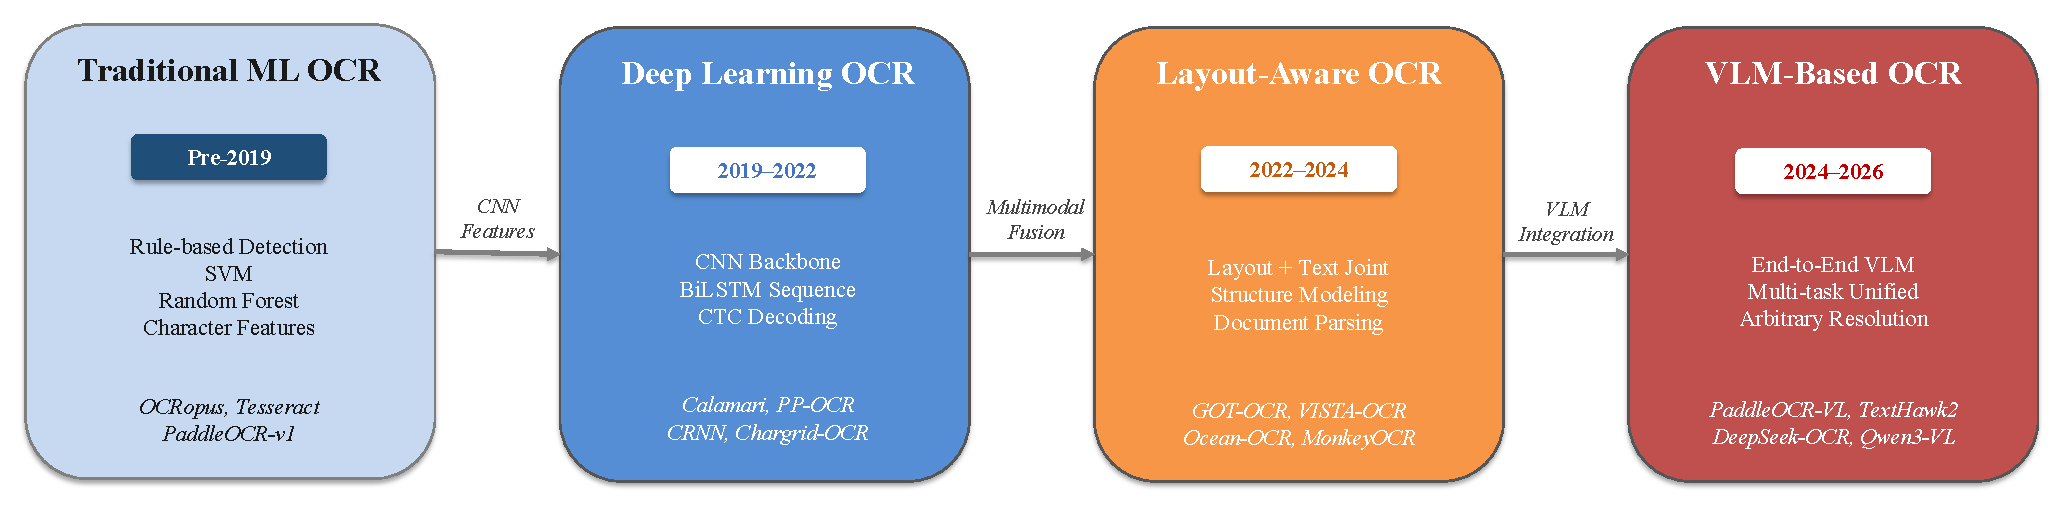
\includegraphics[
    width=0.95\textwidth,
    trim=0cm 0cm 0cm 0cm,
    clip
]{figs_by_qixingyu/fig02.pdf}
\caption{Four-stage evolution of optical character recognition technology (Pre-2019 to 2024--2026): from rule-based Traditional Machine Learning methods, through Deep Learning approaches with CNN--BiLSTM--CTC pipelines, to Layout-Aware OCR with joint structure modeling, and finally to Vision-Language Model-based OCR with end-to-end, multi-task unified frameworks.}
\label{fig:ocr_evolution}
\end{figure*}

\subsubsection{Evaluation}
The evolution of the OCR benchmark evaluation system reflects a profound transition from traditional precision measurement to multi-dimensional capability assessment. The early Fourth Annual Test of OCR Accuracy \cite{rice1994fourth} and Fifth Annual Test of OCR Accuracy \cite{rice1995fifth} established the basic paradigm for systematically evaluating the character-level accuracy of commercial OCR engines, focusing on batch precision testing of standard documents. In the second decade of the 21st century, Performance Comparison of OCR Tools \cite{patel2012performance} continued the traditional approach of tool-level horizontal comparison, while 2022 became a critical turning point: OCR-IDL: OCR Annotations for Industry Document Library Dataset \cite{ocridl2022} provided large-scale commercial OCR annotations for an industrial-grade document library for the first time, pushing evaluation toward real business scenarios; concurrently, an Evaluation of OCR on Egocentric Data \cite{egocentric2022} was among the first to expand OCR capability assessment to the emerging field of first-person perspectives, revealing the limitations of existing methods under non-traditional capture conditions. OCRBench: On the Hidden Mystery of OCR in Large Multimodal Models \cite{ocrbench2023} in 2023 was a milestone, systematically revealing the hidden capability boundaries of large multimodal models across 29 sub-tasks such as text recognition and visual question answering, extending the evaluation dimension from pure character recognition to the level of text understanding and reasoning. The year 2024 saw an explosive development: @BENCH: Benchmarking Vision-Language Models for Human-centered Assistive Technology \cite{atbench2024} incorporated OCR into an assistive technology framework for the visually impaired, emphasizing human-centered utility evaluation; OmniDocBench: Benchmarking Diverse PDF Document Parsing with Comprehensive Annotations \cite{omnidocbench2024} built a refined parsing benchmark covering nine document types; and by year-end, OCRBench v2: An Improved Benchmark for Evaluating Large Multimodal Models on Visual Text Localization and Reasoning \cite{ocrbenchv2_2024} further strengthened the evaluation system for visual text localization and logical reasoning capabilities. Post-2025 development showed three distinct trends: in terms of linguistic diversity expansion, SARD: A Large-Scale Synthetic Arabic OCR Dataset for Book-Style Text Recognition \cite{sard2025} constructed a synthetic dataset of over 840,000 pages for Arabic book-style documents, and 600k-ks-ocr: A Large-Scale Synthetic Dataset for Optical Character Recognition in Kashmiri Script \cite{ksocr2025} filled the resource gap for the endangered Kashmiri script; in terms of refined evaluation dimensions, OCR-Quality: A Human-Annotated Dataset for OCR Quality Assessment \cite{ocrquality2025} introduced a human-annotated quality assessment dimension for the first time, and Real5-OmniDocBench \cite{real5omni2025} focused on robustness evaluation under five types of real physical distortions such as scanning artifacts, bending, and screen photography; in terms of domain specialization, PubMed-OCR: PMC Open Access OCR Annotations \cite{pubmedocr2025} delved into the high-complexity domain of scientific literature, providing dedicated resources for OCR research in academic publications. The entire evolutionary trajectory clearly demonstrates that OCR benchmarks have moved from single character accuracy metrics to a comprehensive evaluation ecosystem encompassing multilingual support, multi-scene adaptation, multi-modal understanding, and real-world robustness, providing critical support for the continuous progress of document intelligence and vision-language models.


\begin{figure*}[t]
\centering
\includegraphics[
    width=0.95\textwidth,
    trim=1.6cm 2.0cm 4.0cm 1.6cm,
    clip
]{figs_by_qixingyu/fig03.pdf}
\caption{Hierarchical summary of representative methods in Document Layout Analysis and OCR, organized by research category and sub-task.}
\label{fig:layout_pipeline1}
\end{figure*}

\begin{figure*}[t]
\centering
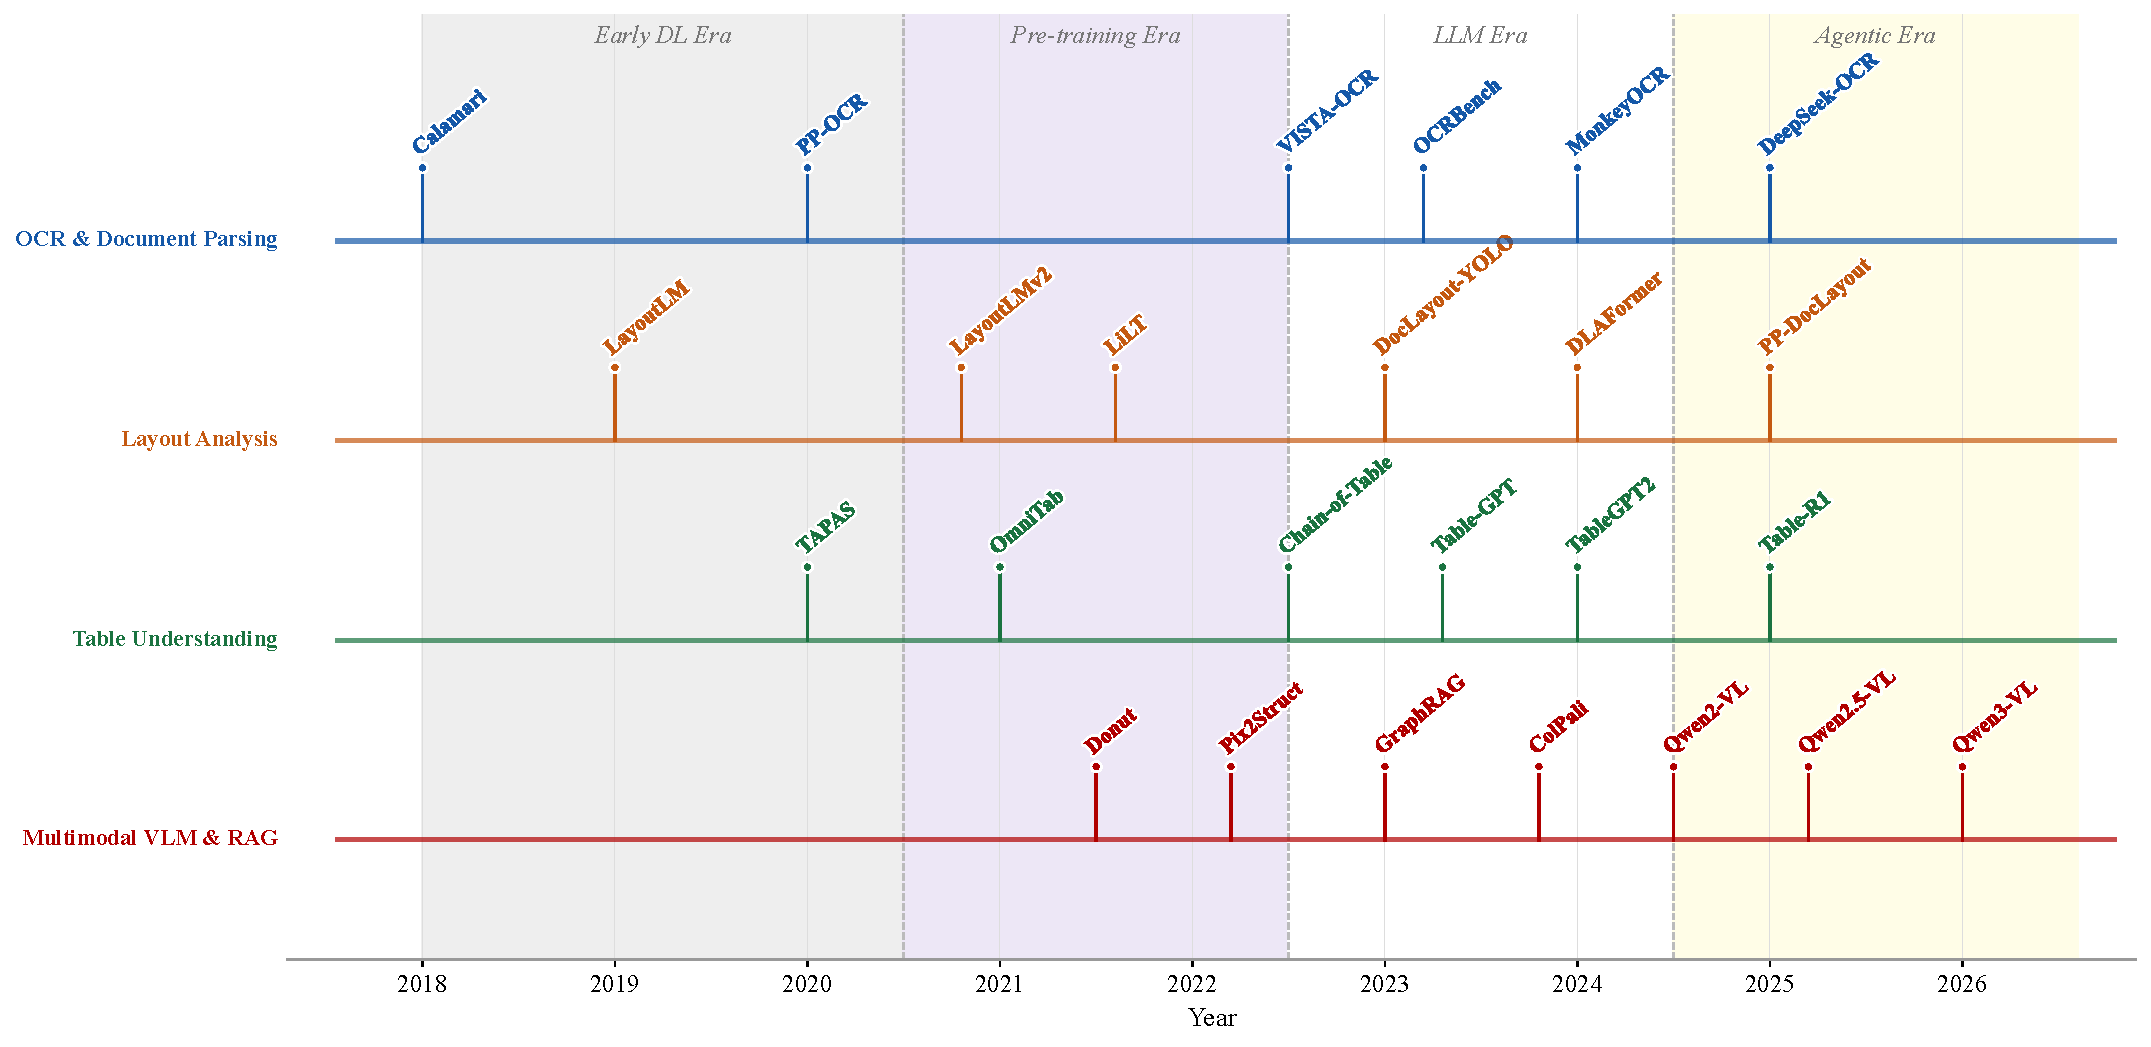
\includegraphics[
    width=0.95\textwidth,
    trim=0cm 0cm 0cm 0cm,
    clip
]{figs_by_qixingyu/fig04.pdf}
\caption{Key method milestones in Document Intelligence (2018--2026) across four research tracks: optical character recognition and document parsing, layout analysis, table understanding, and multimodal vision-language models with retrieval-augmented generation.}
\label{fig:timeline}
\end{figure*}

\section{Document Understanding and Question Answering}

\subsection{Tables}
\subsubsection{Structure-Aware and Table Semantic Modeling Stage}
The research on tables within document understanding and question answering (DocQA) primarily focuses on how models perceive table structures in real-world document scenarios, model the semantic correlations between tables, contextual text, and visual layouts, and provide a reliable representational foundation for subsequent QA and reasoning. Early studies generally recognized that simply linearizing tables into text weakened the ability to model row-column relationships, header hierarchies, and cell dependencies. Consequently, work in this stage concentrated on structure-aware representation learning and the construction of data benchmarks. Understanding Tables with Intermediate Pre-training \cite{eisenschlos2020understanding} and OmniTab \cite{jiang2022omnitab} significantly improved model capabilities in understanding table structures, numerical relationships, and linguistic alignment by introducing large-scale intermediate pre-training and multi-task pre-training. Representations for QA from Documents with Tables and Text \cite{zayats2021representations} and SoarGraph \cite{zhu2023soargraph} further emphasized the joint modeling of tables and their surrounding text, with SoarGraph capturing cross-modal semantic dependencies through graph-structured representations. Furthermore, ReasTAP: Injecting Table Reasoning Skills During Pre-training via Synthetic Reasoning Examples \cite{liu2023reastap} integrated table reasoning capabilities into the pre-training phase, enhancing the model's understanding and reasoning power over tabular data. FORTAP: Using formulas for numerical-reasoning-aware table pretraining \cite{cheng2022fortap} leveraged spreadsheet formulas to achieve numerical-reasoning-aware table pre-training, providing support for computational capabilities on unstructured tables. At the task and data level, AIT-QA \cite{katsis2022ait}, FeTaQA \cite{nan2022fetaqa}, and Arxiv Tables \cite{konopka2023arxiv} revealed the limitations of traditional methods in real-world scenarios from the perspectives of complex industry tables, free-form table QA, and long-document table-text associations, respectively, and constructed related datasets. Meanwhile, Table Detection in the Wild: A Novel Diverse Table Detection Dataset and Method \cite{li2021tablewild} provided a large-scale table detection dataset and benchmark methods, laying the groundwork for subsequent table structure modeling. As research expanded to visual documents, Visual Understanding of Complex Table Structures from Document Images \cite{raja2022visual} and HTAN \cite{wu2025htan} proposed more robust visual structure modeling methods for irregular and hierarchical tables, while Towards Complex Document Understanding by Discrete Reasoning \cite{zhu2022towards} and RJUA-MedDQA \cite{jin2024rjua} further evaluated table understanding within the context of multi-page, multimodal documents and complex discrete reasoning. Additionally, from an analytical perspective, Tabular Representation, Noisy Operators, and Impacts on Table Structure Understanding Tasks in LLMs \cite{singha2023tabular} and Large Language Models Are Complex Table Parsers \cite{zhao2023large} revealed the sensitivity of LLMs to table representation formats and structural noise, pointing out that their table parsing capabilities were still constrained by input structure and robustness bottlenecks.  Overall, research in this stage systematically established the theoretical and methodological foundations for structure-aware representation learning in table document understanding, providing a critical prerequisite for the development of subsequent generative reasoning and verifiable table QA methods.

\subsubsection{Generation Enhancement and Modular Reasoning Stage}
After completing the fundamental modeling of table structures and cross-modal representations, the research focus gradually shifted toward leveraging the generative capabilities of LLMs to improve the answerability and generalization of complex table QA through modular, decomposed, and generation-enhanced strategies. One representative category of work centered on table instruction tuning and generation-capability enhancement. Table-GPT \cite{peng2023table} performed "table-tuning" on general-purpose LLMs using large-scale synthetic table task data, enabling the models to gain stronger transfer capabilities across multiple table tasks. TableGPT2 \cite{su2024tablegpt2} further introduced specialized table encoders and multimodal pre-training to mitigate the deficiencies in structural and semantic modeling of complex real-world tables, while Rethinking Table Instruction Tuning \cite{deng2025rethinking} systematically analyzed the impact of hyperparameters and training scales on performance and generalization in table instruction tuning. Another important route focused on the modular organization of the generation process: Localize, Retrieve and Fuse (TAG-QA) \cite{zhao2023localize} supported free-form table QA through a three-stage "localize-retrieve-fuse" framework; Open-Domain Question Answering over Tables with LLMs \cite{liang2024open} extended this idea to open-domain scenarios with large-scale table collections. MFORT-QA \cite{guan2024mfort} combined few-shot learning with multi-hop Chain-of-Thought (CoT) to handle cross-table and complex reasoning problems, while Large Language Models are Versatile Decomposers \cite{ye2023large} explicitly proposed using LLMs as question and evidence decomposers, alleviating issues of large table input redundancy and unclear reasoning paths through a "decompose-then-reason" approach. Regarding input organization and noise suppression, TACR \cite{wu2024table} utilized table-question alignment to achieve fine-grained cell selection; CABINET \cite{patnaik2024cabinet} reduced interference from irrelevant table content through unsupervised relevance scoring; TabSQLify: Enhancing reasoning capabilities of LLMs through table decomposition \cite{nahid2024tabsqlify} reduced context length burdens by decomposing large tables into question-relevant sub-tables; and GENTAP \cite{shi2022generation} enhanced model performance in free-form table QA through generation-oriented intermediate pre-training. Meanwhile, Exploring the Impact of Table-to-Text Methods \cite{min2024exploring} systematically compared the effectiveness of different table-to-text strategies in DSFT and RAG scenarios. DocTabQA \cite{wang2024doctabqa} introduced generation-enhancement ideas into long-document scenarios, improving the clarity of complex information presentation through tabular answer organization.

In the exploration of finer-grained table reasoning methods, Chain-of-table: Evolving tables in the reasoning chain for table understanding \cite{zhang2023chainoftable} proposed integrating tabular data into the reasoning chain to enhance table understanding. DePlot: One-shot visual language reasoning by plot-to-table translation \cite{liu2023deplot} achieved visual language reasoning through plot-to-table translation. MultiHiertt: Numerical reasoning over multi hierarchical tabular and textual data \cite{wang2023multihiertt} provided a numerical reasoning benchmark and symbolic reasoning QA model for multi-hierarchical tables and text. Alter: Augmentation for large-table-based reasoning \cite{kim2023alter} improved large-table reasoning capabilities through data and query augmentation. Towards table-to-text generation with numerical reasoning \cite{gao2023tabletotext} focused on the numerical reasoning aspect of generating text from structured data. Effective distillation of table-based reasoning ability from LLMs \cite{chen2023tablellmdistill} proposed distilling the table reasoning capabilities of large models into smaller ones. Tables as texts or images: Evaluating the table reasoning ability of LLMs and MLLMs \cite{singh2023tablesastext} evaluated table understanding under different prompting strategies and data formats. Tap4llm: Table provider on sampling, augmenting, and packing semi-structured data for large language model reasoning \cite{liu2024tap4llm} provided a toolkit for table preprocessing. Table as Thought: Exploring Structured Thoughts in LLM Reasoning \cite{huang2023tableasthought} proposed organizing the reasoning process in tabular form to enhance LLM reasoning power. RoT: Enhancing Table Reasoning with Iterative Row-Wise Traversals \cite{xu2023rot} optimized reasoning efficiency through iterative row-wise traversals. Improving table reasoning through table decomposition and normalization \cite{li2023tabulardecompose} optimized table reasoning via decomposition and normalization. FLEXTAF: Enhancing Table Reasoning with Flexible Tabular Formats \cite{wang2024flextaf} strengthened reasoning performance with flexible tabular formats. VisTR: Visualizations as Representations for Time-series Table Reasoning \cite{zhang2024vistr} supported time-series table reasoning via visualization. LIGHT-TABLE-CHAIN: Simplifying and Enhancing Chain-Based Table Reasoning \cite{chen2024lighttablechain} optimized the efficiency of chain-based table reasoning. Reasoning and retrieval for complex semi-structured tables via reinforced relational data transformation \cite{liu2023tabformer} proposed the TabFormer framework to achieve semi-structured table reasoning and retrieval. Beyond Linearization: Attributed Table Graphs for Table Reasoning \cite{gao2024attributedtablegraph} used attributed table graphs to preserve structural information for graph-structured reasoning. TableReasoner: Advancing Table Reasoning Framework with Large Language Models \cite{singh2024tablereasoner} utilized LLMs to advance table reasoning frameworks. STaR: Towards Cognitive Table Reasoning via Slow-Thinking Large Language Models \cite{wang2024starcognitive} optimized multi-step reasoning and stability through a slow-thinking approach. PanelTR: Zero-Shot Table Reasoning Framework Through Multi-Agent Scientific Discussion \cite{liu2024paneltr} proposed a multi-agent zero-shot table reasoning framework. Table-Critic: A Multi-Agent Framework for Collaborative Criticism and Refinement in Table Reasoning \cite{zhang2024tablecritic} improved table reasoning capabilities by identifying and correcting reasoning errors through multi-agent collaboration. Unveiling Implicit Table Knowledge with Question-Then-Pinpoint Reasoner for Insightful Table Summarization \cite{kim2024qtp} excavated implicit table knowledge via self-questioning and evidence pinpointing. Tab-CoT: Zero-shot Tabular Chain of Thought \cite{li2024tabcot} achieved zero-shot tabular Chain-of-Thought reasoning.

\subsubsection{Verifiable Reasoning and Multimodal Table Understanding Stage}
After generation enhancement and modular reasoning methods significantly expanded the coverage of table QA systems for complex questions, recent research has begun to focus further on the verifiability of the reasoning process itself, execution consistency, and cross-modal reliability. This focus aims to build interpretable table understanding and QA systems with engineering robustness in real-world table and complex document scenarios. Among representative works, Table-R1: Inference-Time Scaling for Table Reasoning \cite{yang2025tablegpt1} proposed an inference-time scaling method for table reasoning, improving performance across various table reasoning tasks through post-training strategies. Weaver: Interweaving SQL and LLM for Table Reasoning \cite{weaver2025} combined SQL with LLMs to dynamically process structured and unstructured data via a modular pipeline to enhance QA capabilities. Tart: An open-source tool-augmented framework for explainable table-based reasoning \cite{tart2024} proposed a tool-augmented framework to improve LLM interpretation of tabular data. Meanwhile, Reasoning-Table: Exploring Reinforcement Learning for Table Reasoning \cite{reasoningtable2025} designed a reinforcement learning-based table reasoning model, validating its effectiveness in tasks such as table QA and text-to-SQL. Concurrently, TableGPT-R1 \cite{yang2025tablegpt} introduced reinforcement learning into table reasoning, mitigating the limitations of supervised fine-tuning in multi-step reasoning and code execution through task-adaptive rewards and multi-stage training. Interpretable LLM-based Table QA \cite{nguyen2024interpretable} proposed Plan-of-SQLs (POS), which explicitly decomposes natural language queries into executable SQL sub-steps to achieve end-to-end verifiable reasoning. Multi-LLM Agent QA over Tabular Data \cite{bangar-etal-2025-exploration} completed planning, code generation, and debugging through multi-agent collaboration, demonstrating the feasibility of agentic reasoning in table QA.

In the direction of tool and execution enhancement, OpenTab \cite{kong2024opentab} combined table retrieval with SQL execution to support open-domain table reasoning. TAT-LLM \cite{zhu2024tat} and MATATA \cite{vinayagame2025matata} strengthened discrete and mathematical reasoning capabilities in hybrid table-text scenarios through a step-wise pipeline and a weakly supervised tool-augmentation mechanism, respectively. TaPERA \cite{zhao2024tapera} significantly improved the trustworthiness and consistency of long-form table QA through a content planning and execution-driven reasoning workflow. Table-r1: Region-based reinforcement learning for table understanding \cite{tabler12025} proposed a region-level reinforcement learning method, optimizing table understanding by fusing regional evidence with advanced fine-tuning techniques. PoTable: Towards Systematic Thinking via Stage-oriented Plan-then-Execute Reasoning on Tables \cite{potable2024} introduced a stage-oriented plan-then-execute strategy to enhance reasoning systematicity and interpretability. Potable: Programming standardly on table-based reasoning like a human analyst \cite{potable2025} simulated human analytical thinking by combining a planner with a Python interpreter to achieve complex computational tasks. TableMind: An Autonomous Programmatic Agent for Tool-Augmented Table Reasoning \cite{tablemind2025} strengthened structured table reasoning capabilities through a multi-stage training strategy. JT-DA: Enhancing Data Analysis with Tool-Integrated Table Reasoning Large Language Models \cite{jt-da2025} provided a complete analysis and reasoning workflow to support complex table QA. Fortune: Formula-Driven Reinforcement Learning for Symbolic Table Reasoning in Language Models \cite{fortune2025} enhanced the symbolic reasoning power of LLMs by generating executable spreadsheet formulas.

Meanwhile, interpretability and structural consistency have been systematically reinforced in visual table scenarios. TabIQA \cite{nguyen2023tabiqa}, ExpliCIT-QA \cite{hormazabal2025explicit}, Enhancing LVLMs with Layout Modality \cite{aida2025enhancing}, and Extracting Information from Scientific Literature via Visual Table QA Models \cite{kim2024extracting} emphasized the importance of maintaining table structure and execution trajectories from the perspectives of structural recovery, code-interpretable reasoning, layout-aware modeling, and scientific literature extraction, respectively. TabPedia \cite{zhao2024tabpedia} and Compositional Condition QA \cite{jiangcompositional} further improved multimodal consistent reasoning through unified multi-task visual table understanding and condition-aware modeling. From the perspective of external knowledge and structural constraints, From Liberating to Questioning Tabular Data using Knowledge Graphs \cite{raj2024liberating} and TQAgent \cite{zhao2025tqagent} integrated knowledge graphs into table QA to reduce hallucinations and support multi-step tree-like reasoning. Finally, TReB \cite{li2025treb} provided a systematic evaluation framework spanning shallow understanding to deep reasoning, revealing the gaps in existing methods for real-world complex table reasoning. Overall, this stage centered on execution, verification, and structural alignment, pushing table QA from "generating answers" to making "answers interpretable, reproducible, and trustworthy," marking a significant transition in table document understanding research toward engineering usability and high-stakes applications.

\begin{figure*}[t]
\centering
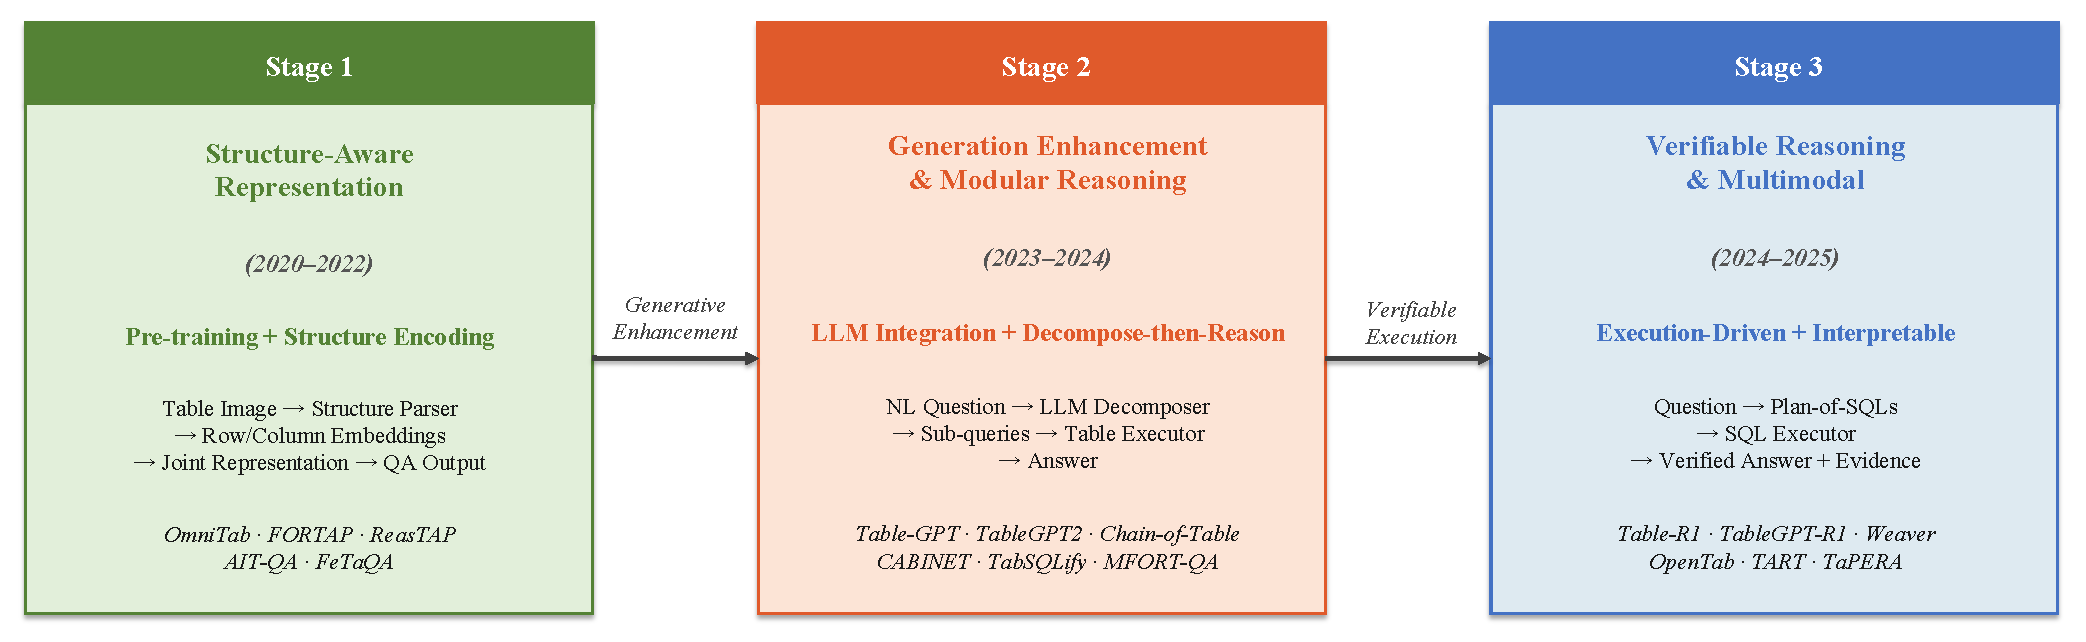
\includegraphics[
    width=0.95\textwidth,
    trim=0cm 0cm 0cm 0cm,
    clip
]{figs_by_qixingyu/fig05.pdf}
\caption{Three-stage evolution of table understanding and question answering (2020--2025): Stage~1 establishes structure-aware representation learning via pre-training and structure encoding; Stage~2 advances generation enhancement and modular reasoning through LLM integration and decompose-then-reason strategies; Stage~3 achieves verifiable reasoning and multimodal understanding driven by execution and interpretable inference.}
\label{fig:table_stages}
\end{figure*}
\subsection{Text-Based Retrieval-Augmented Generation}
\subsubsection{Retrieval-Augmented Generation}

Early research on document-level question answering (DocQA) faced two core challenges: first, Large Language Models (LLMs) were limited by context length, making it difficult to directly process long or multi-document inputs; second, pure generative models were prone to hallucinations when lacking external evidence constraints, performing unstably in fact-dense scenarios or those requiring cross-document reasoning. Against this backdrop, researchers initially proposed the Retrieval-Augmented Generation (RAG) paradigm, which combines information retrieval with text generation. Its core intuition was to first retrieve evidence relevant to the question from an external document collection and then guide the language model to generate an answer within a controlled context, thereby enhancing factual coverage and answer reliability without significantly increasing the model size. Early RAG primarily followed the classic "retrieve-then-generate" paradigm, which improved DocQA performance by enhancing evidence recall quality and multi-hop support capabilities. Triple-Fact Retriever \cite{wu2022triple} improved the accuracy and interpretability of cross-document evidence paths in multi-hop DocQA by extracting structured triple facts and aggregating evidence hop by hop. Multi-Document Question Answering with Lightweight Embeddings-based Document Reranker \cite{aitymbetov2024multi} employed a two-stage retrieval process combining BM25 coarse-ranking with lightweight embedding-based re-ranking, improving evidence quality in multi-document QA while maintaining efficiency. Zero-Shot Complex Question-Answering on Long Scientific Documents \cite{wang2025zero} integrated RAG with question decomposition, multi-hop reasoning, and long-answer generation, achieving complex QA on long documents without task-specific fine-tuning. Meanwhile, DR-RAG \cite{hei2024dr} mitigated evidence omission in multi-hop QA caused by static similarity retrieval by introducing dynamic document relevance modeling and a two-stage filtering mechanism.

Building on traditional RAG improvements centered on retrieval quality and multi-hop support, subsequent research began to focus further on utilizing the reasoning capabilities of LLMs and internal or cross-document structural information to construct more structure-aware and reasoning-guided retrieval-augmentation frameworks. Among these, DocReLM: Mastering Document Retrieval with Language Model \cite{wei2024docrelm} fine-tuned retrievers and re-rankers by introducing LLMs to generate domain-specific training data and utilized LLM-generated citation networks to expand candidate document sets, thereby significantly enhancing semantic understanding and cross-literature association discovery in academic literature retrieval. Advanced Chain-of-Thought Reasoning for Parameter Extraction from Documents Using Large Language Models \cite{chen2025advanced} introduced an improved chain-of-thought reasoning mechanism into document-level information extraction tasks, achieving reasoning-driven refined retrieval and parameter localization through modules such as Targeted Document Retrieval, Iterative Retrieval Optimization, and Preference Optimization. Semi-Structured Chain-of-Thought: Integrating Multiple Sources of Knowledge for Improved Language Model Reasoning \cite{su2024semi} further explored the unification of parametric knowledge, structured knowledge graphs, and unstructured text retrieval into a semi-structured reasoning chain, allowing multi-source knowledge to be progressively filled and integrated during the reasoning process. In long-document scenarios, Beyond Chunking: Discourse-Aware Hierarchical Retrieval for Long Document Question Answering \cite{chen2025chunkingdiscourseawarehierarchicalretrieval} utilized Rhetorical Structure Theory (RST) for discourse-level modeling of documents and performed hierarchical retrieval on this structure, effectively alleviating the issue of semantic incoherence caused by flat chunking. For multi-document scenarios, Knowledge Graph Prompting for Multi-Document Question Answering \cite{wang2024knowledge} enhanced global consistency and multi-document reasoning capabilities by constructing cross-document knowledge graphs and guiding the LLM through graph-traversal evidence collection. Meanwhile, PdfTriage: Question Answering over Long, Structured Documents \cite{saad2024pdftriage} focused on structured long-document QA, explicitly modeling structural meta-information such as pages, sections, and tables to enable RAG to accurately respond to queries containing structural references. Overall, work in this stage marked the evolution of RAG from "similarity-centric retrieval augmentation" to a "document-level information acquisition paradigm driven jointly by structure and reasoning."

Despite the significant improvements in evidence localization and multi-document understanding achieved by the aforementioned works through document structure, knowledge graphs, and reasoning-guided retrieval, their overall processes still largely relied on preset retrieval strategies. The connection between retrieval and reasoning was often a "retrieve-then-reason" sequence, making it difficult to dynamically adjust retrieval paths, depth, and evidence combinations as reasoning unfolds. In long-document, multi-hop, and multi-document QA scenarios, this static retrieval mode still readily resulted in broken evidence chains, accumulation of redundant information, or omission of critical evidence. To address this, subsequent RAG research further treated "retrieval" as a decision-making step directly driven and scheduled by the reasoning process: First, From Local to Global: A Graph RAG Approach to Query-Focused Summarization \cite{edge2024graphrag} (GraphRAG) proposed a graph-enhanced retrieval framework based on knowledge graphs and community detection, achieving precise understanding and comprehensive answers for global, cross-document queries by constructing entity-relationship graphs and generating hierarchical community summaries. Subsequently, LightRAG: Simple and Fast Retrieval-Augmented Generation \cite{guo2024lightrag} addressed the high computational overhead of GraphRAG by designing a lightweight dual-level index architecture, significantly reducing indexing time and storage costs while retaining the semantic advantages of graph structures, thus enhancing reasoning efficiency and facilitating the industrial deployment of graph-enhanced RAG. Furthermore, HyperGraphRAG: Retrieval-Augmented Generation via Hypergraph-Structured Knowledge Representation \cite{he2024hypergraphrag} broke through the theoretical limitations of traditional binary graphs by introducing hypergraph structures to directly model n-ary relations, preserving the semantic integrity of complex events by connecting multiple entities through a single hyperedge, thus achieving more accurate knowledge retrieval and generation in scenarios highly dependent on n-ary relationship reasoning, such as medical and legal fields. Leveraging Spreading Activation for Improved Document Retrieval in Knowledge-Graph-Based RAG Systems \cite{pavlovic2025leveraging} enabled activation values to propagate dynamically along evidence chains for prioritized retrieval of relevant fragments by automatically constructing knowledge graphs and executing spreading activation, serving as a plug-and-play module that enhanced multi-hop evidence continuity in chain-based reasoning. GARLIC: LLM-Guided Dynamic Progress Control with Hierarchical Weighted Graph for Long Document QA \cite{wang2024garlic} constructed a hierarchical weighted directed acyclic graph based on LLM attention for dynamic retrieval, allowing retrieval paths and information volume to be adaptively controlled by the LLM, overcoming the limitations of traditional vector similarity and fixed tree summarization. For multi-document environments, HiQA: A Hierarchical Contextual Augmentation RAG for Multi-Documents QA \cite{chen2024hiqa} transformed documents into hierarchical structures with cascading metadata and fused vector, BM25, and keyword matching through multi-path retrieval to improve retrieval discriminability in structurally similar document sets. For complex hierarchical documents, BookRAG: A Hierarchical Structure-aware Index-based Approach for Retrieval-Augmented Generation on Complex Documents \cite{wang2025bookrag} built BookIndex, fusing logical hierarchy trees and entity-relationship graphs, and introduced an agentic retrieval strategy inspired by information foraging theory to dynamically select retrieval workflows, thereby balancing recall, efficiency, and multi-hop path integrity. In multi-hop reasoning, Enhancing Document-Level Question Answering via Multi-Hop Retrieval-Augmented Generation with LLaMA 3 \cite{huang2025enhancing} integrated dense retrieval, context fusion, and multi-hop mechanisms, strengthening retrieval-generation synergy through the joint optimization of retrieval likelihood and generation loss. Finally, Chain of Retrieval: Multi-Aspect Iterative Search Expansion and Post-Order Search Aggregation for Full Paper Retrieval \cite{park2025chain} drove iterative expansion retrieval via multi-aspect decomposition and reorganized hierarchical evidence through post-order aggregation, reflecting a paradigm shift in which the retrieval process itself served as the reasoning chain. Overall, work in this stage marked the further evolution of RAG from "structure-aware retrieval augmentation" to a modular retrieval and generation framework dynamically driven by the reasoning process.

\begin{figure*}[t]
\centering
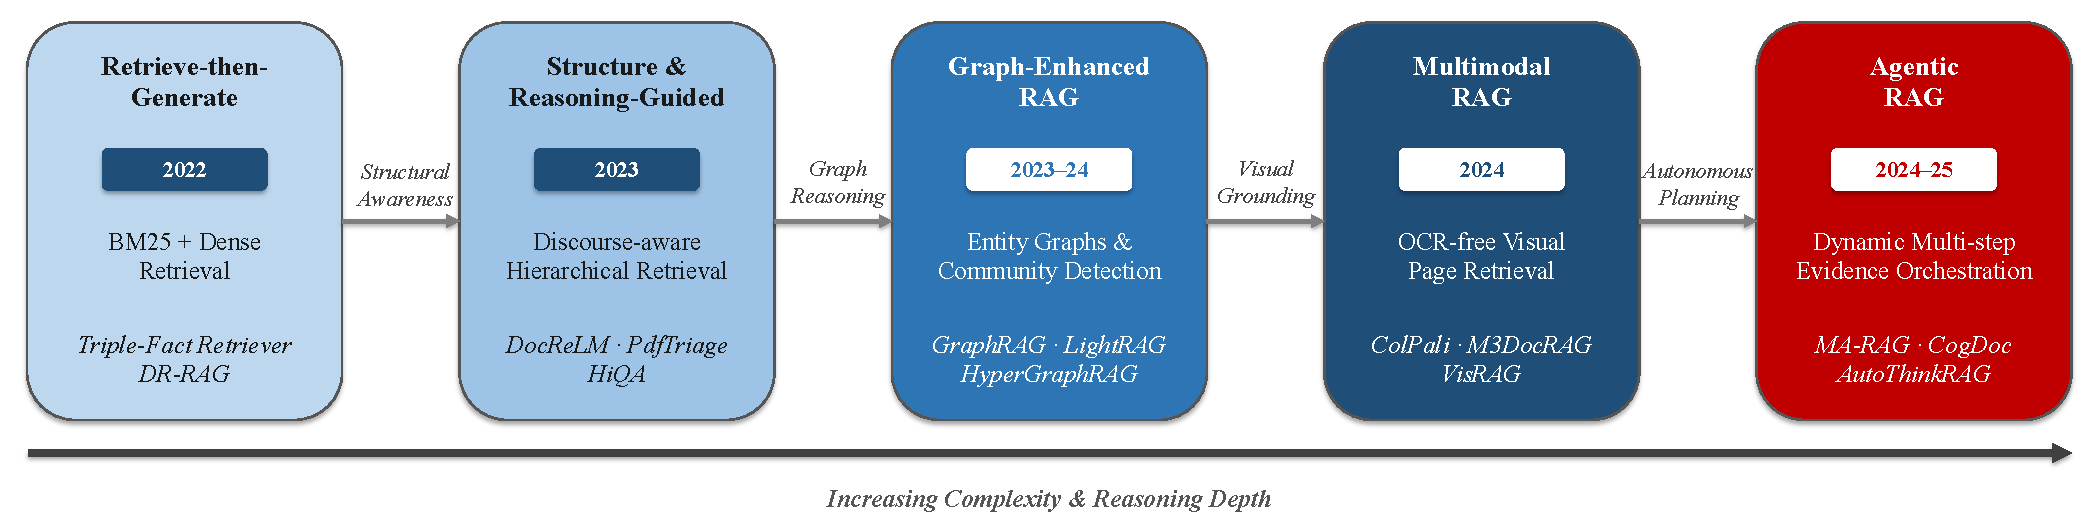
\includegraphics[
    width=0.95\textwidth,
    height=0.38\textheight,
    keepaspectratio,
    trim=0cm 0cm 0cm 0cm,
    clip
]{figs_by_qixingyu/fig06.pdf}
\caption{Five-stage evolution of retrieval-augmented generation paradigms for document question answering, progressing from Retrieve-then-Generate (2022) through Structure and Reasoning-Guided RAG (2023), Graph-Enhanced RAG (2023--2024), Multimodal RAG (2024), and Agentic RAG (2024--2025), with representative systems listed at each stage and increasing complexity and reasoning depth indicated along the horizontal axis.}
\label{fig:rag_evolution}
\end{figure*}

\subsubsection{End-to-End Document Question Answering}

\paragraph{Early Attention Mechanisms}
Document understanding originated with the construction of attention mechanisms to capture context. Dynamic Coattention Networks \cite{dynamiccoattention2017} proposed a co-attention strategy to capture bidirectional interaction information by simultaneously attending to the question and the document. Addressing the excessive search range in long documents, Coarse-to-fine question answering \cite{coarsetofine2017} pioneered a "coarse-to-fine" two-stage framework: first retrieving relevant sentences, then extracting precise answers. To further enhance text representation capabilities, EA Reader \cite{eareader2019} utilized multi-space context fusion to improve performance in cloze-style QA.

\paragraph{Reasoning Based on Graph Structures and Global Information}
As document length and complexity continued to increase, Graph Neural Networks (GNNs) became the core paradigm for connecting discrete pieces of evidence. Question Answering by Reasoning Across Documents with GCNs \cite{gcnmultihop2019} was among the earliest works to utilize entity-based Graph Convolutional Networks for handling multi-hop tasks. Subsequently, Identifying Supporting Facts with Document Graph Networks \cite{dgn2019} further shifted the research focus from answer prediction to the explicit identification of supporting facts. This shift was achieved by modeling multi-document contexts as sentence-level document graphs and introducing question-conditioned GNN reasoning mechanisms on the graph structure. Meanwhile, the Heterogeneous Graph approach \cite{heterograph2019} handled cross-document reasoning by modeling different types of nodes (e.g., entities, documents). In recent research, Path-based GCN \cite{pathgcn2020} emphasized reasoning along specific relational paths, while Capturing global structural information in long document question answering with compressive graph selector network \cite{cgsn2022} achieved more efficient long-document QA through integrated global structural encoding.

To improve the capability and interpretability of multi-hop QA, researchers began exploring explicit reasoning chains and explainable frameworks. First, Exploiting Explicit Paths \cite{explicitpaths2019} proposed that the key lay in selecting a correct evidence path, with the model scoring and choosing within a path space. Multi-hop Question Answering via Reasoning Chains \cite{reasoningchains2020} proposed the use of "reasoning chains" as intermediate explicit variables, where the model predicted one or more reasoning chains before generating an answer. Explore, Propose, and Assemble \cite{epa2019} proposed a three-stage explainable reasoning framework to bridge information fragments. Further progress in explainability included Select, Answer and Explain \cite{sae2020}, which simultaneously generated answers and evidence rationales, elevating "explanation" from an auxiliary task to an output as important as the answer itself. Hop, Union, Generate \cite{hug2023} proposed guiding the model to form an explainable reasoning process without explicit evidence supervision. Additionally, Ask to Understand \cite{asktounderstand2023} proposed revealing complex multi-hop logic clearly by generating a series of intermediate questions.

\paragraph{Task Generalization and the LLM Era}
Methods such as multi-hop reasoning expanded from pure QA to broader document-level tasks. Multi-Hop Transformer \cite{multihoptransformer2021} explicitly introduced multi-hop reasoning into the translation field for the first time. Syntax-enhanced multi-hop reasoning networks \cite{syntaxmultihop2024} advanced document-level relation extraction by introducing syntactic structures as reasoning constraints, where multi-hop reasoning progressively aggregated evidence under syntactic guidance. DocScript \cite{docscript2024} applied multi-hop logic to script event prediction, treating events as nodes and modeling the evolutionary relationships between events through multi-hop logical reasoning. Regarding the efficiency of ultra-long texts, MemSum-DQA \cite{memsumdqa2023} streamlined the input of QA models by improving extractive summarizers, significantly compressing input length while preserving the evidence integrity required for multi-hop reasoning. Finally, as the field entered the Large Language Model (LLM) era, the latest research, such as Effect of Document Packing \cite{documentpacking2025}, began to explore in depth the potential multi-hop reasoning capabilities of LLMs and how document organization (packing) affected their reasoning performance.

\subsection{Vision-Language Models for Document Understanding}
\subsubsection{Foundational Vision-Language Models for Document Understanding}
The development of Vision-Language Models (VLM) has propelled visual document understanding from single-modality analysis toward a unified multimodal modeling paradigm. By jointly modeling visual content, textual semantics, and spatial layout information, VLMs enable systems to gain a deeper understanding of document structures and their semantic relationships. Building on this capability, visual document understanding has gradually evolved into a general intelligent system characterized by structure awareness, cross-modal reasoning, and document-level understanding. The following sections introduce the evolution of VLMs across four key dimensions.

\paragraph{Foundational Period of Visually-Rich Document Understanding}
Early research established the technical foundations for document image classification and cross-modal retrieval.
Deep multimodal learning for cross-modal retrieval: One model for all tasks \cite{wei2020deep} proposed a "unified model" approach, encoding vision and text into the same retrievable representation space to simultaneously support bidirectional image-text retrieval and unimodal retrieval within a single model.
Entering the pre-training era, Layoutxlm: Multimodal pre-training for multilingual visually-rich document understanding \cite{xu2021layoutxlm} introduced a multimodal pre-training model for multilingual, visually-rich documents, integrating text, layout, and visual information into a unified multilingual pre-training framework.
VinVL: Revisiting Visual Representations in Vision-Language Models \cite{zhang2021vinvl} systematically investigated the role of "visual features themselves" in multimodal tasks, proving that high-quality visual encoding is a key factor in enhancing VLM performance.
CLIP-Adapter: Better Vision-Language Models with Feature Adapters \cite{gao2021clipadapter} proposed an efficient way to adapt CLIP without compromising its pre-training capabilities by adding lightweight ``adapter'' modules in the feature space to improve performance on few-shot and downstream tasks.
In 2022, the research community began focusing on constructing generalized document processors.
FLAVA: A Foundational Language And Vision Alignment Model \cite{singh2022flava} presented a foundational model for general vision-language understanding, proposing the use of both image-text pairs and unimodal data for pre-training under a unified Transformer architecture to balance cross-modal alignment and unimodal understanding.
Unifying Vision, Text, and Layout for Universal Document Processing \cite{li2022udop} proposed the UDOP framework, which models visual appearance, textual content, and spatial layout in documents as a unified sequence-to-sequence generative task, supporting various document understanding and generation tasks through an instructional prompt mechanism.
Unified Pretraining Framework for Document Understanding \cite{wang2022unified} proposed a unified document pre-training framework that performs large-scale pre-training by multimodally encoding semantic regions in documents and combining multiple self-supervised learning objectives, thereby improving model transfer and generalization across different document understanding tasks.
Bi-VLDoc: Bidirectional Vision-Language Modeling for Visually-Rich Document Understanding \cite{yang2022bivldoc} designed a bidirectional vision-language supervision mechanism, enabling the model to predict language from vision and vice versa, strengthening cross-modal alignment and semantic interaction.
Multimodal pre-training based on graph attention network for document understanding \cite{liu2022gatdoc} explicitly modeled document structure as a graph and performed multimodal pre-training based on Graph Attention Networks, allowing the model to better capture contextual dependencies driven by layout relationships.
CM3: A Causal Masked Multimodal Model of the Internet \cite{ai2022cm3} adopted a generative multimodal pre-training strategy using causal masking, modeling text and image tokens in a unified sequence to provide the model with both multimodal understanding and generation capabilities.
NLX-GPT: A Model for Natural Language Explanations in Vision and Vision-Language Tasks \cite{kayser2022nlxgpt} introduced a unified model for simultaneously predicting answers and generating natural language explanations in vision and vision-language tasks.
Furthermore, Vision and natural language for metadata extraction from scientific PDF documents: a multimodal approach \cite{li2022pdfmeta} proposed a multimodal method merging visual layout and textual semantics to automatically extract structured metadata from scientific PDF documents.
I2MVFormer: Large Language Model Generated Multi-View Document Supervision for Zero-Shot Image Classification \cite{zhao2022i2mvformer} utilized Large Language Models to generate multi-view textual descriptions as supervision signals, enhancing semantic modeling in zero-shot image and document classification.

\paragraph{The Rise of VLM and Advancements in High-Resolution Perception}
With the integration of Large Language Models (LLMs), document understanding entered an instruction-driven phase.
PaLM-E: An Embodied Multimodal Language Model \cite{driess2023palme} proposed an embodied multimodal language model, enabling language models to directly process inputs from various sensors and achieve integrated modeling of visual, linguistic, and embodied reasoning tasks.
MiniGPT-4: Enhancing Vision-Language Understanding with Advanced Large Language Models \cite{zhu2023minigpt4} explored how advanced LLMs can improve vision-language understanding by aligning features from a frozen visual encoder with a powerful pre-trained LLM (such as Vicuna) using only a single projection layer, significantly enhancing visual description and text generation while retaining visual and linguistic capabilities.
PaLI-X: On Scaling up a Multilingual Vision and Language Model \cite{chen2023palix} introduced a large-scale multilingual VLM that achieved significant performance gains in multilingual image captioning, visual question answering, document understanding, and few-shot learning by scaling component sizes and task diversity.
mPLUG-PaperOwl: Scientific Diagram Analysis with the Multimodal Large Language Model \cite{ye2023paperowl} focused on enhancing the understanding and analysis of scientific diagrams by general multimodal LLMs, significantly outperforming existing models in multimodal diagram description, analysis, and outline recommendation, demonstrating powerful capabilities in deep scientific diagram parsing and opening new directions for academic content generation.
Additionally, UniDoc: A Universal Large Multimodal Model for Simultaneous Text Detection, Recognition, Spotting and Understanding \cite{li2023unidoc} proposed a unified multimodal large model framework capable of end-to-end text detection, recognition, spotting, and semantic understanding within a single model---a holistic capability previously unavailable in similar methods.
Between 2023 and 2024, high-resolution processing became the core focus.
Monkey: Image Resolution and Text Label Are Important Things for Large Multimodal Models \cite{li2024monkey} systematically studied the impact of image resolution and text label quality on MLLM performance, noting that in document understanding and text-dense scenarios, resolution improvements often yield more direct and significant gains than structural changes, as high-resolution input markedly improves the perception of fine-grained text, symbols, and layout structures.
TextMonkey: An OCR-Free Large Multimodal Model for Understanding Documents \cite{li2024textmonkey}, building on the analysis of Monkey, proposed an end-to-end OCR-free document understanding model that performs joint visual and semantic modeling directly from high-resolution document images.
Qwen2-VL: Enhancing Vision-Language Model's Perception of the World at Any Resolution \cite{wang2024qwen2vl} addressed the instability of VLM perception under different resolution conditions by proposing a unified modeling framework supporting arbitrary resolution inputs.
DocKylin: A Large Multimodal Model for Visual Document Understanding with Efficient Visual Slimming \cite{liu2024dockylin} focused on the computational overhead brought by high-resolution inputs, proposing an efficient visual slimming strategy that maintains document understanding performance while significantly reducing the number of visual tokens.
DocPedia: Unleashing the Power of Large Multimodal Model in the Frequency Domain for Versatile Document Understanding \cite{zhao2023docpedia} explored the potential value of frequency-domain information in visual document understanding, breaking the traditional paradigm that relies almost exclusively on spatial-domain features by merging frequency-domain representations with spatial features to better capture repetitive textures and structural patterns.
Meanwhile, Vary: Scaling up the Vision Vocabulary for Large Vision-Language Models \cite{huang2023vary} argued from the perspective of visual representation discretization that existing VLMs face expression bottlenecks in visual vocabulary scale, requiring a systematic expansion of the visual vocabulary to allow the model to express complex image content with finer-grained visual tokens.
DocLLM: A layout-aware generative language model for multimodal document understanding \cite{wang2024docllm} proposed an explicitly layout-aware generative language model that directly integrates spatial structure information into the language generation process, ensuring generated results align with the document's structural logic and semantic organization.
mPLUG-DocOwl 1.5: Unified Structure Learning for OCR-free Document Understanding \cite{hu2024mplugdocowl15} further strengthened structure learning capabilities under an OCR-free framework, proposing a unified structure modeling mechanism to capture relationships between text, layout, and visual cues.
For chart-centric document scenarios, TinyChart-3B \cite{zhang2024tinychart} demonstrated that specialized lightweight MLLMs can achieve strong structural and numerical reasoning by combining visual token merging with Program-of-Thoughts learning, thereby attaining high chart understanding performance with only 3B parameters.
Qwen-VL: A Versatile Vision-Language Model for Understanding, Localization, Text Reading, and Beyond \cite{bai2023qwenvl} introduced a highly versatile VLM framework supporting image understanding, region localization, text reading, and cross-modal reasoning, performing exceptionally well in text-dense and complex layout scenarios.
Furthermore, document understanding for small models has gained attention.
PaLI-3 Vision Language Models: Smaller, Faster, Stronger \cite{chen2023pali3} achieved stronger multimodal understanding at a smaller model scale through architectural design and training strategy optimization, greatly expanding application scenarios.
Small Language Model Meets with Reinforced Vision Vocabulary \cite{li2024slmrvv} explored the potential of Small Language Models (SLMs) in multimodal contexts, proposing to compensate for limited model scale by reinforcing the vision vocabulary. By enhancing the expressive power on the visual side, small models significantly improved their performance in document understanding and visual reasoning, approaching the level of large models in certain scenarios.
To optimize alignment, Enhancing Visual Document Understanding with Contrastive Learning in Large Visual-Language Models \cite{wu2024contrastivedoc} introduced contrastive learning objectives to enhance the alignment between visual and textual representations, thereby mitigating semantic mismatch issues in complex documents.
Read and Think: An Efficient Step-wise Multimodal Language Model for Document Understanding and Reasoning \cite{lu2024readthink} proposed a stepwise multimodal reasoning framework that decomposes document understanding into sequential reading and reasoning stages, improving the model's ability to handle long documents and complex questions while maintaining computational efficiency.
Gemini: A Family of Highly Capable Multimodal Models \cite{team2023gemini} introduced a family of unified multimodal large models covering text, images, audio, and video. In visual document understanding scenarios, Gemini demonstrated powerful cross-modal reasoning and contextual integration capabilities.
VisionLLM v2: An End-to-End Generalist Multimodal Large Language Model for Hundreds of Vision-Language Tasks \cite{wang2024visionllmv2} unified a vast array of vision-language tasks in an end-to-end manner, emphasizing versatility and scalability. In document understanding, it showed stable cross-task generalization, representing the trend toward general-purpose multimodal models.
EVLM: An Efficient Vision-Language Model for Visual Understanding \cite{li2024evlm} optimized visual encoding and cross-modal fusion modules from a holistic system efficiency perspective, balancing performance and computational cost across various tasks.
3MVRD: Multimodal Multi-task Multi-teacher Visually-Rich Form Document Understanding \cite{zhang2024mmvrd} proposed a multimodal, multi-task, multi-teacher distillation framework for joint modeling of visually-rich documents. Through collaborative guidance from multiple teachers, the model showed stronger generalization in multi-task scenarios, reflecting the effectiveness of knowledge transfer in document understanding.
A LayoutLMv3-Based Model for Enhanced Relation Extraction in Visually-Rich Documents \cite{li2024layoutlmv3re} reinforced relation extraction in visually-rich documents based on LayoutLMv3, highlighting the role of layout information in structured semantic modeling and proving that explicit layout modeling can effectively improve the accuracy of entity relationship understanding.
\begin{figure*}[t]
\centering
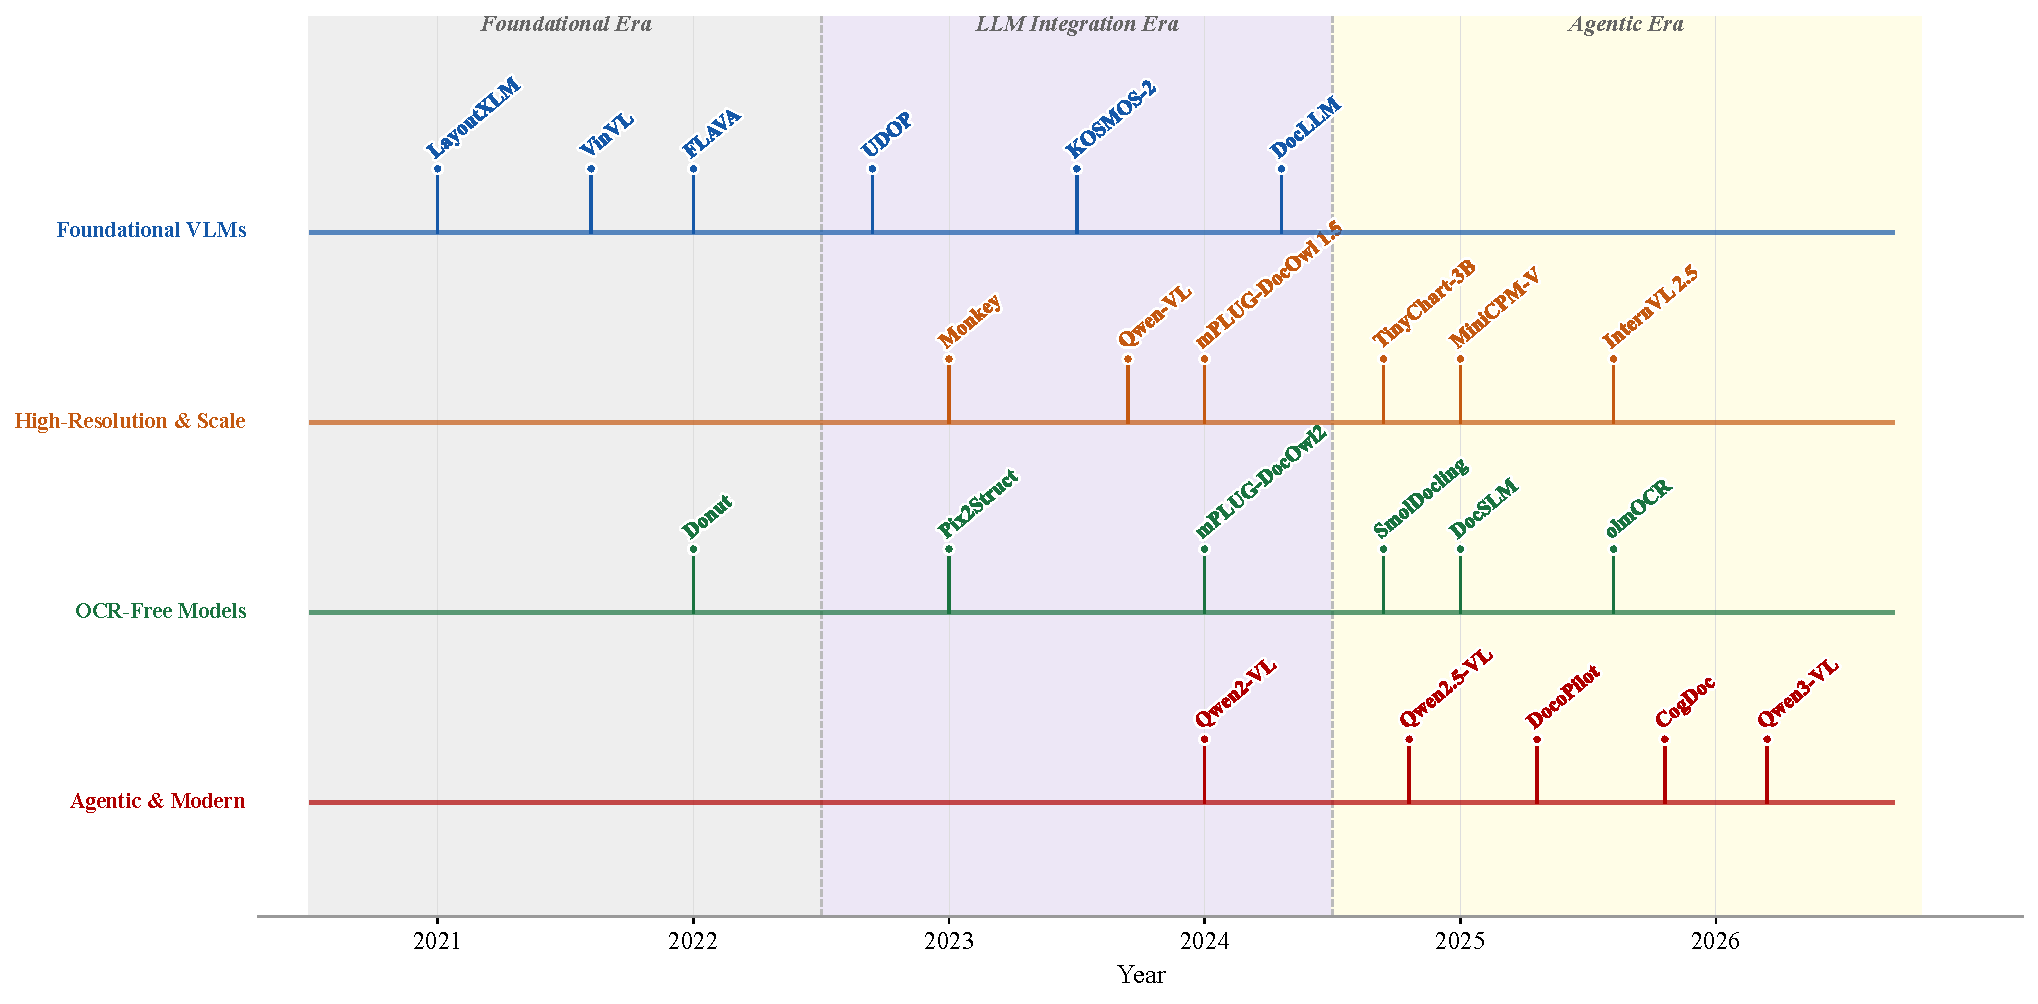
\includegraphics[
    width=0.95\textwidth,
    trim=0cm 0cm 0cm 0cm,
    clip
]{figs_by_qixingyu/fig07.pdf}
\caption{Evolution of vision-language models for document understanding (2021--2026)---organized into four development tracks: foundational vision-language models, high-resolution and scaled architectures, OCR-free models, and agentic systems for complex document reasoning.}
\label{fig:vlm_evolution}
\end{figure*}

\paragraph{The Evolution of OCR-free and Multi-page Context}
Moving away from traditional OCR dependency and handling long documents are key steps toward the practicality of VRDU. Traditional document understanding methods usually rely on Optical Character Recognition (OCR) systems to convert document images into text before performing semantic analysis. However, this process disconnects "text recognition" and "document understanding" into two independent steps; if OCR makes an error or structural information is lost, subsequent models struggle to recover the original semantics. OCR-free models utilize joint vision-language modeling, taking raw document images as direct input, using visual encoders to extract features, and using structures like Transformers to generate text or structured results in an end-to-end fashion. Such an approach allows the model to implicitly learn character and semantic information without explicitly calling an OCR system. This unified modeling avoids OCR error propagation and more completely preserves the layout and visual context, showing stronger robustness and generalization in complex layouts, multi-page documents, and cross-modal understanding tasks.
OCR-free Document Understanding Transformer (Donut) \cite{kim2022donut} was an end-to-end document understanding model that did not rely on OCR systems. Based on a Transformer encoder-decoder structure, it generates structured text output directly from raw document images, avoiding error propagation in traditional OCR pipelines. Experimental results show that Donut achieves competitive performance across various tasks while significantly simplifying the document processing workflow.
Pix2Struct \cite{lee2023pix2struct} proposed an OCR-free VLM based on screenshot parsing pre-training, capable of generating structured text representations directly from raw images using a Transformer encoder-decoder architecture to achieve unified vision-language understanding.
mPLUG-DocOwl: Modularized Multimodal Large Language Model for Document Understanding \cite{ye2023docowl} introduced a modularized MLLM for OCR-free document understanding to address the issue of existing models ignoring fine-grained visual features in complex scenarios, demonstrating stronger cross-task generalization even without specific fine-tuning.
mPLUG-DocOwl2: High-resolution Compressing for OCR-free Multi-page Document Understanding \cite{ye2024docowl2} proposed an efficient visual compression and structural modeling method for multi-page documents to address the computational and contextual bottlenecks in OCR-free scenarios. This model compresses and aggregates cross-page visual information while maintaining high-resolution perception, significantly reducing visual token counts and supporting long-document modeling.
DeepSeek-VL2: Mixture-of-Experts Vision-Language Models for Advanced Multimodal Understanding \cite{deepseek2024vl2} adopted the Mixture-of-Experts (MoE) architecture in VLMs, significantly improving parameter efficiency through an expert routing mechanism that dynamically activates sub-models for different types of visual and semantic inputs.
Regarding complex document parsing, MinerU2.5 \cite{liu2025mineru25} proposed an efficient high-resolution document parsing framework. It employs a coarse-to-fine two-stage parsing strategy to address computational bottlenecks: the first stage performs global layout analysis on downsampled images to identify structural elements, while the second stage crops key regions based on the global layout.
POINTS-Reader: Distillation-Free Adaptation of Vision-Language Models for Document Conversion \cite{wang2025pointsreader} proposed a distillation-free adaptation framework focusing on the lack of high-quality annotated data in complex document conversion tasks.
PDF-WuKong: A Large Multimodal Model for Efficient Long PDF Reading with End-to-End Sparse Sampling \cite{li2024pdfwukong} addressed the challenges of merging large-scale visual and textual information in long PDF documents by selecting paragraphs or charts most relevant to user queries, avoiding redundant computation of the entire document.
LongFin: A Multimodal Document Understanding Model for Long Financial Domain Documents \cite{chen2024longfin} introduced a model specifically designed for multimodal understanding of long financial documents, breaking the maximum length limits of traditional models to accommodate multi-page, long-content industrial financial documents.
Furthermore, H2OVL-Mississippi Vision Language Models Technical Report \cite{h2ovl2024mississippi} introduced a suite of small VLMs aimed at meeting the needs for efficient, lightweight document processing in privacy-sensitive and on-device scenarios.
FILA: Fine-Grained Vision Language Models \cite{liu2024fila} focused on the fine-grained visual understanding capabilities of MLLMs when processing high-resolution images, providing a solution to the object truncation and semantic fragmentation issues caused by dynamic cropping and re-encoding.
Expanding Performance Boundaries of Open-Source Multimodal Models with Model, Data, and Test-Time Scaling \cite{chen2024internvl25} presented the InternVL 2.5 series, systematically studying the impact of model scale, data quality, and test-time strategies on MLLM performance and providing a deep analysis of each factor's contribution to multimodal understanding.
Additionally, Multimodal Adaptive Inference for Document Image Classification with Anytime Early Exiting \cite{sun2024anytime} proposed a multimodal adaptive inference framework to balance efficiency and performance in VRDU tasks by embedding multi-layer early exiting mechanisms within the base model.

\paragraph{Modern Document Understanding Evolution}
The years 2025 and 2026 witnessed an explosion of ultra-lightweight models.
DocSLM: A Small Vision-Language Model for Long Multimodal Document Understanding \cite{wang2025docslm} proposed an efficient small VLM to address the computational and memory bottlenecks of large-scale VLMs in long document understanding and edge deployment, achieving or exceeding state-of-the-art performance with significantly fewer parameters.
SmolDocling: An ultra-compact vision-language model for end-to-end multimodal document conversion \cite{kim2025smoldocling} focused on end-to-end multimodal document conversion, proposing an extremely compact VLM that processes complete pages within a single network and expresses all elements and their positions through a universal tagging format called DocTags.
Specific applications and vertical domain research include Baseer: A Vision-Language Model for Arabic Document-to-Markdown OCR \cite{albaseer2025baseer}, which designed a specialized VLM for the unique challenges of Arabic OCR and fine-tuned it on a mixed dataset of synthetic and real documents to accurately convert Arabic documents into structured Markdown.
IndoColSmol: Lightweight Vision-Language Models for Multimodal Indonesian Document Search \cite{rahman2025indocolsmol} proposed two lightweight vision-language retrieval models focused on multimodal retrieval tasks for Indonesian documents.
Semantic Document Derendering: SVG Reconstruction via Vision-Language Modeling \cite{kim2025derendering} introduced a multimodal-based vectorization tool to parse complex document images into editable vector formats.
Qwen2.5-VL Technical Report \cite{bai2025qwen25vl} established performance benchmarks for unified vision-language understanding, localization, and text reading.
Qwen3-VL Technical Report \cite{bai2025qwen3vl} further expanded model capacity and reasoning capabilities, enhancing cross-modal task generalization and fine-grained perception.
Finally, document-level strategy research includes Docopilot: Improving Multimodal Models for Document-Level Understanding \cite{duan2025docopilot}, which addressed the shortcomings of MLLMs in multi-page document-level tasks by proposing a native document-level multimodal large model framework to replace retrieval-augmented generation methods.
Nayana: A Foundation for Document-Centric Vision-Language Models via Multi-Task \cite{kolavi2025nayana} aimed to build a multi-task, multimodal, and multilingual foundational resource and training framework, significantly expanding the potential of VLMs in global document understanding scenarios.
PP-DocBee2: Improved Baselines with Efficient Data for Multimodal Document Understanding \cite{du2025docbee2} proposed a set of foundational enhancement strategies for end-to-end document image understanding.
Interpret, prune and distill Donut: towards lightweight VLMs for VQA on document \cite{zhou2025donutdistill} focused on compressing generative VLMs like Donut into lightweight versions using interpretation, pruning, and distillation for efficient Document VQA.
LoRA-Contextualizing Adaptation of Large Multimodal Models for Long Document Understanding \cite{li2025loracontext} introduced LoRA structures to VLMs, allowing the model to serve as an efficient base for self-visual retrieval-augmented generation frameworks while adapting to long-document tasks through fine-grained parameter adjustments.
SCoPE VLM: Selective Context Processing for Efficient Document Navigation in Vision-Language Models \cite{wang2025scopevlm} proposed a strategy called "Chain of Scroll" for selective and recursive navigation in long documents to avoid the high memory consumption of processing full pages at once.
Entering 2026, A Hybrid Architecture for Multi-Stage Claim Document Understanding: Combining Vision-Language Models and Machine Learning for Real-Time Processing \cite{patel2026claim} proposed a multi-stage hybrid architecture for the automated processing of medical and insurance claim documents, designing an end-to-end pipeline to handle challenges like mixed layouts, handwriting, and diverse languages in scanned or photographed documents.

\subsubsection{Multimodal RAG}
Building on the success of text RAG in pure text QA, researchers began extending the retrieval-augmented paradigm to Visual Document Question Answering (DocQA/DocVQA), forming an early multimodal transition path centered on OCR/structural parsing + text retrieval. This stage generally assumed that document semantics primarily stem from text, using OCR to convert visual documents into text and layout structures before expanding retrieval and generation capabilities. PDF-MVQA \cite{ding2024mvqa} noted the bias of existing benchmarks toward single-page sparse text and constructed a multi-page visually-rich document QA dataset, proposing a joint coarse-to-fine retrieval framework for cross-page localization. CREAM \cite{zhang2024cream} introduced a coarse-to-fine retrieval pipeline and merged multi-page visual encoding to address evidence sparsity and retrieval efficiency in long contexts. DocLLM \cite{wang2024docllm} mitigated the neglect of text-layout relationships in traditional VLMs by explicitly modeling spatial layout, improving the stability of generative DocQA. ViTLP \cite{mao2024visually} jointly modeled text and layout during pre-training, enabling the model to handle long documents without relying on ultra-long contexts. Overall, this series of work established the OCR + text RAG paradigm centered on textual evidence with layout and vision as aids, providing a key transition for subsequent OCR-free and deeper multimodal fusion methods.

As the "OCR + text retrieval" method exposed issues of structural and visual information loss in visually-rich documents, research shifted toward OCR-free visual retrieval paradigms, completing retrieval and alignment directly in the original visual space of the document. ColPali \cite{faysse2024colpali} proposed a page-level OCR-free document retrieval method, using VLMs to generate multi-vector page representations and achieving multi-granularity matching between queries and pages through a late-interaction mechanism, significantly improving retrieval robustness for complex layouts while introducing the ViDoRe benchmark to systematically evaluate OCR-free retrieval. Document Screenshot Embedding \cite{ma2024unifying} further used document screenshots as a unified retrieval input, jointly encoding text, images, and layout into dense vectors through large VLMs, allowing a single retrieval system to adapt to various document forms.

After OCR-free page retrieval began solving visual structure fidelity and cross-modal alignment, multimodal RAG research moved toward a stage centered on multi-page, multi-document, multimodal evidence fusion and reasoning consistency. The focus shifted from "whether relevant pages can be retrieved" to "how to organize, align, and verify scattered evidence in complex document collections." Representative works like VisRAG \cite{yu2024visrag} and VDocRAG \cite{tanaka2025vdocrag} were pioneers in introducing VLMs to the retrieval stage, using the overall visual representation of a page or document to drive generation, laying the foundation for cross-chart and cross-layout QA. M3DocRAG \cite{cho2024m3docrag} systematically proposed multi-page, multi-document, multimodal DocQA tasks and significantly improved cross-document evidence coverage by integrating visual cues into the RAG workflow. Subsequent research deepened at the level of evidence organization and reasoning: CMRAG \cite{chen2025cmrag} mitigated unimodal bias through dual-channel retrieval of text and images; RegionRAG \cite{li2025regionrag} lowered retrieval granularity to the region level to reduce visual noise; MHier-RAG \cite{gong2025mhier} integrated fragmented cross-page evidence with hierarchical indexing; MoLoRAG \cite{wu2025molorag} and QCG-RAG \cite{wu2025query} introduced logic-aware and query-driven graph structures to enhance multi-hop reasoning; and HKRAG \cite{tong2025hkrag} improved answer completeness through holistic modeling of salient knowledge and fine-grained details. Furthermore, Luminirag \cite{martis2024luminirag} and MMGraphRAG \cite{wan2025mmgraphrag} unified vision and text into graph structures for structured cross-modal retrieval and interpretable reasoning. AutoThinkRAG \cite{autothinkrag} further advanced this line by introducing a query-complexity-aware router that dynamically allocates retrieval and reasoning paths, enabling more efficient multimodal DocQA under long and information-dense document settings. In addition, AutoThinkRAG proposed a decoupled perception-and-reasoning paradigm, where a lightweight VLM first translates query-relevant visual evidence into textual descriptions and an LLM subsequently performs logical synthesis, alleviating the reasoning bottleneck of end-to-end VLMs. TableRAG \cite{yu2025tablerag} extended this to heterogeneous text-table documents, maintaining structural semantics through retrieval combined with programmatic execution. VisDoM \cite{suri2025visdom} and ViDoRAG \cite{wang2025vidorag} utilized multi-step or multi-agent reasoning to improve evidence combination across multiple documents. Finally, Look as You Think \cite{liu2025look} and RAG-Anything \cite{guo2025rag} advanced this line further from the perspectives of verifiable reasoning and unified knowledge representation, with the former using reinforcement learning to achieve precise attribution of reasoning steps and visual evidence, and the latter integrating all-modality knowledge with dual-graph structures. This stage marks the transition of multimodal RAG from "retrieval-augmented generation" to a systematic framework of "evidence orchestration, reasoning consistency, and verifiability," providing a more robust and interpretable path for real-world complex DocQA.

\subsubsection{Agentic Frameworks for Document QA}
In recent years, research on multi-document and long-document QA has shifted from static RAG to agentic reasoning frameworks with process modeling capabilities. Early work relied on concatenating document snippets as input to LLMs, which suffered from deficiencies in evidence integration, reasoning controllability, and hallucination suppression. CuriousLLM \cite{yang2025curiousllm}, based on Knowledge Graph Prompting (KGP) and graph traversal agents, introduced a curiosity-driven follow-up question generation mechanism. This allows the model to actively guide retrieval and expand evidence coverage, mitigating the loss of reasoning direction in multi-document QA while reducing the computational and latency overhead of the original KGP methods.
In visually-rich long document scenarios, simple text-level retrieval struggles to locate key evidence. DocLens \cite{zhu2025doclens} proposed a tool-enhanced multi-agent framework for long visual document understanding, achieving step-by-step focusing from the entire document to key pages and visual elements through explicit page-level zooming (Lens) and a sampling-judging mechanism, showing significant improvements over traditional long-context strategies.
From a more general RAG perspective, MA-RAG \cite{nguyen2025ma} pointed out that a single retrieval-generation process struggles with query ambiguity and evidence sparsity. It introduced a multi-agent system with a clear division of labor, decoupling question decomposition, retrieval control, evidence extraction, and answer synthesis through collaborative chain-of-thought communication to systematically improve multi-hop QA performance.
For collection-level retrieval and reasoning of visual documents, ViDoRAG \cite{wang2025vidorag} proposed a dynamic iterative reasoning agent. By using hybrid multimodal retrieval strategies and an exploration-reflection workflow, it strengthened joint reasoning of visual and textual evidence and provided the ViDoSeek benchmark to address the lack of evaluation for large-scale visual document collections.
Further targeting "research-level" complex queries, Doc-Researcher \cite{dong2025doc} unified multimodal document parsing, dynamic multi-granularity retrieval, and multi-agent reasoning into an end-to-end system, emphasizing evidence chain accumulation and cross-modal consistency, with systematic evaluation of multi-hop and multi-round capabilities via M4DocBench.
Parallel agent research also includes visual agents for interactive environments. CogAgent \cite{hong2024cogagent} built a VLM-based agent capable of understanding and navigating interfaces directly from high-resolution screen pixels, demonstrating the scalability of agentic visual understanding in non-document environments.
At the methodological level, HEAR \cite{chen2025hear} explicitly introduced agentic reasoning into the document understanding process, establishing coordination between information extraction and reasoning generation to organize multimodal evidence actively.
Finally, CogDoc \cite{xu2025cogdoc} proposed a unified coarse-to-fine thinking paradigm based on cognitive modeling. Through a two-stage coordination of fast localization and deep reasoning, combined with reinforcement learning for strategy optimization, it mitigates fine-grained semantic loss while maintaining scalability.

\begin{figure*}[t]
\centering
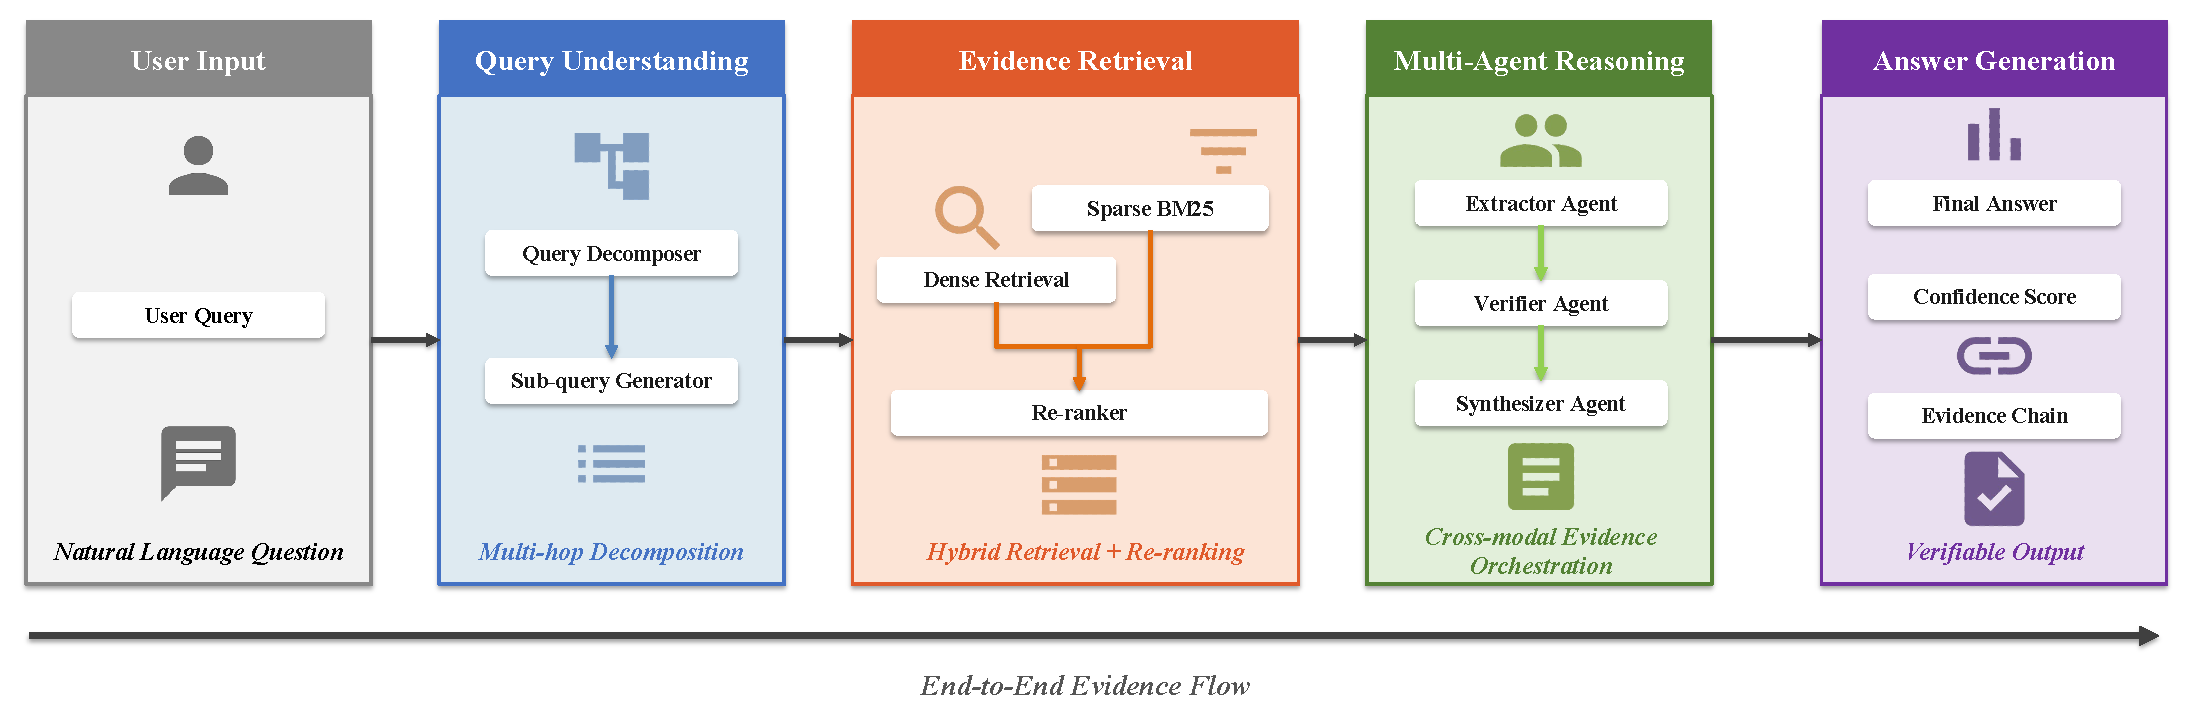
\includegraphics[
    width=0.95\textwidth,
    height=0.40\textheight,
    keepaspectratio,
    trim=0cm 0cm 0cm 0cm,
    clip
]{figs_by_qixingyu/fig08.pdf}
\caption{Agentic Document QA pipeline illustrating end-to-end evidence flow: a user natural language query passes through Query Understanding (multi-hop decomposition), Evidence Retrieval (hybrid dense and sparse retrieval with re-ranking), Multi-Agent Reasoning (extractor, verifier, and synthesizer agents for cross-modal evidence orchestration), and Answer Generation (producing a final answer with an evidence chain and confidence score).}
\label{fig:agent_docqa}
\end{figure*}
\subsection{Evaluation}
With the advancement of Large Language Models (LLMs), the performance of models in complex document processing and Retrieval-Augmented Generation (RAG) tasks has become a central focus of research.


\subsubsection{Visual Document Understanding and Basic QA Evaluation}

\begin{figure*}[t]
    \centering
    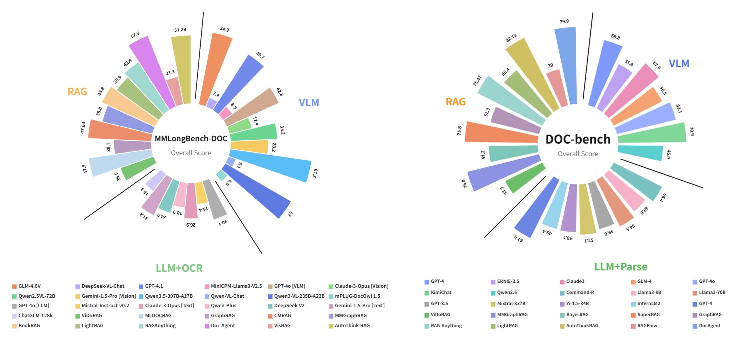
\includegraphics[page=1,width=\textwidth]{figs_by_qixingyu/fig09.pdf}
    \caption{Performance comparison of representative models on MMLongBench-Doc and DocBench, two benchmarks for evaluating multimodal long-document understanding.}
    \label{fig:combined}
\end{figure*}
Document Question Answering (DocQA) research primarily focuses on whether models can correctly understand text, layout, and visual cues from single-page or small-scale documents. DocVQA~\cite{docvqa2020} is one of the earliest benchmarks to systematically propose "question answering on document images," emphasizing the localization of facts by understanding text, layout, and visual cues in single-page documents. Document Collection VQA~\cite{doccollectionvqa2021} for the first time placed questions in a document collection scenario, requiring models to locate answers across multiple documents. InfographicVQA~\cite{infographicvqa2021} focuses on infographic QA to evaluate the model's understanding and reasoning capabilities in mixed scenarios of complex layouts, charts, and text. A Dataset of Information-Seeking Questions and Answers Anchored in Research Papers~\cite{infoseekqa2021} proposed a QA dataset oriented toward long scientific research papers, focusing on the types of questions readers actually ask while reading. DUE: End-to-End Document Understanding Benchmark~\cite{due2021} proposed a comprehensive benchmark for end-to-end document understanding, where models start from raw documents, obtain text and layout through OCR and layout modeling, and then complete downstream tasks. These datasets primarily focus on visual text understanding, region localization, and factual QA in single documents or small-scale collections, laying the most fundamental input and evaluation paradigm for subsequent "Retrieval + Reasoning."

Next, the research focus began to shift from "understanding one page" to "cross-page understanding and localization." Hierarchical Multimodal Transformers for Multi-Page DocVQA \cite{tito2023hierarchicalmultimodaltransformersmultipage} was the first to systematically handle multi-page documents, answering "what to do when information is scattered across multiple pages" through hierarchical structural modeling of pages and document-level semantics. VRDU~\cite{vrdu2023} proposed a "Visually Rich Document Understanding" benchmark and evaluation framework specifically for complex business document information extraction tasks in real business scenarios. Test-Time Adaptation for Visual Document Understanding~\cite{tta-vdu2023} is oriented toward visual document understanding, enabling models to adapt to new documents at test time.

Simultaneously, datasets with the problem setting of "locating evidence from a large number of pages" began to emerge. PDFVQA~\cite{pdfvqa2023} introduced real PDF documents into evaluation for the first time, where questions often require locating key information among many pages. SlideVQA~\cite{slidevqa2023} is a DocVQA dataset for multi-page slide documents consisting of slide images and natural language questions, used to study understanding and reasoning across multiple image pages. DUDE~\cite{dude2023} is a document understanding benchmark and evaluation framework proposed in 2023, oriented toward DocVQA and comprehensive document understanding evaluation on visually rich documents. DLUE \cite{dlue2023} is a comprehensive evaluation dataset and task suite for long and complex-structured documents, used to systematically assess model capabilities in document-level language understanding. KNVQA \cite{knvqa2023} proposed a knowledge-based visual QA evaluation dataset and benchmark, primarily used to assess the "factuality" and knowledge reasoning abilities of Large Vision-Language Models (LVLMs). Privacy-Aware Document VQA \cite{privacydocvqa2023} is a privacy-sensitive dataset and benchmark for DocVQA, used to study automatic QA and information extraction on real invoices under Federated Learning and Differential Privacy constraints, revealing the constraints of DocQA in real-world applications and pushing evaluation from ideal to reality. PDFTriage \cite{saad2024pdftriage} is a QA benchmark and methodology for long structured documents (e.g., PDFs), used to evaluate and enhance the QA capabilities of large models in "whole book / ultra-long context" scenarios, with a particular emphasis on the role of document structure (chapters, page numbers, tables, images, etc.) in retrieval and answering.

\begin{figure*}[t]
\centering
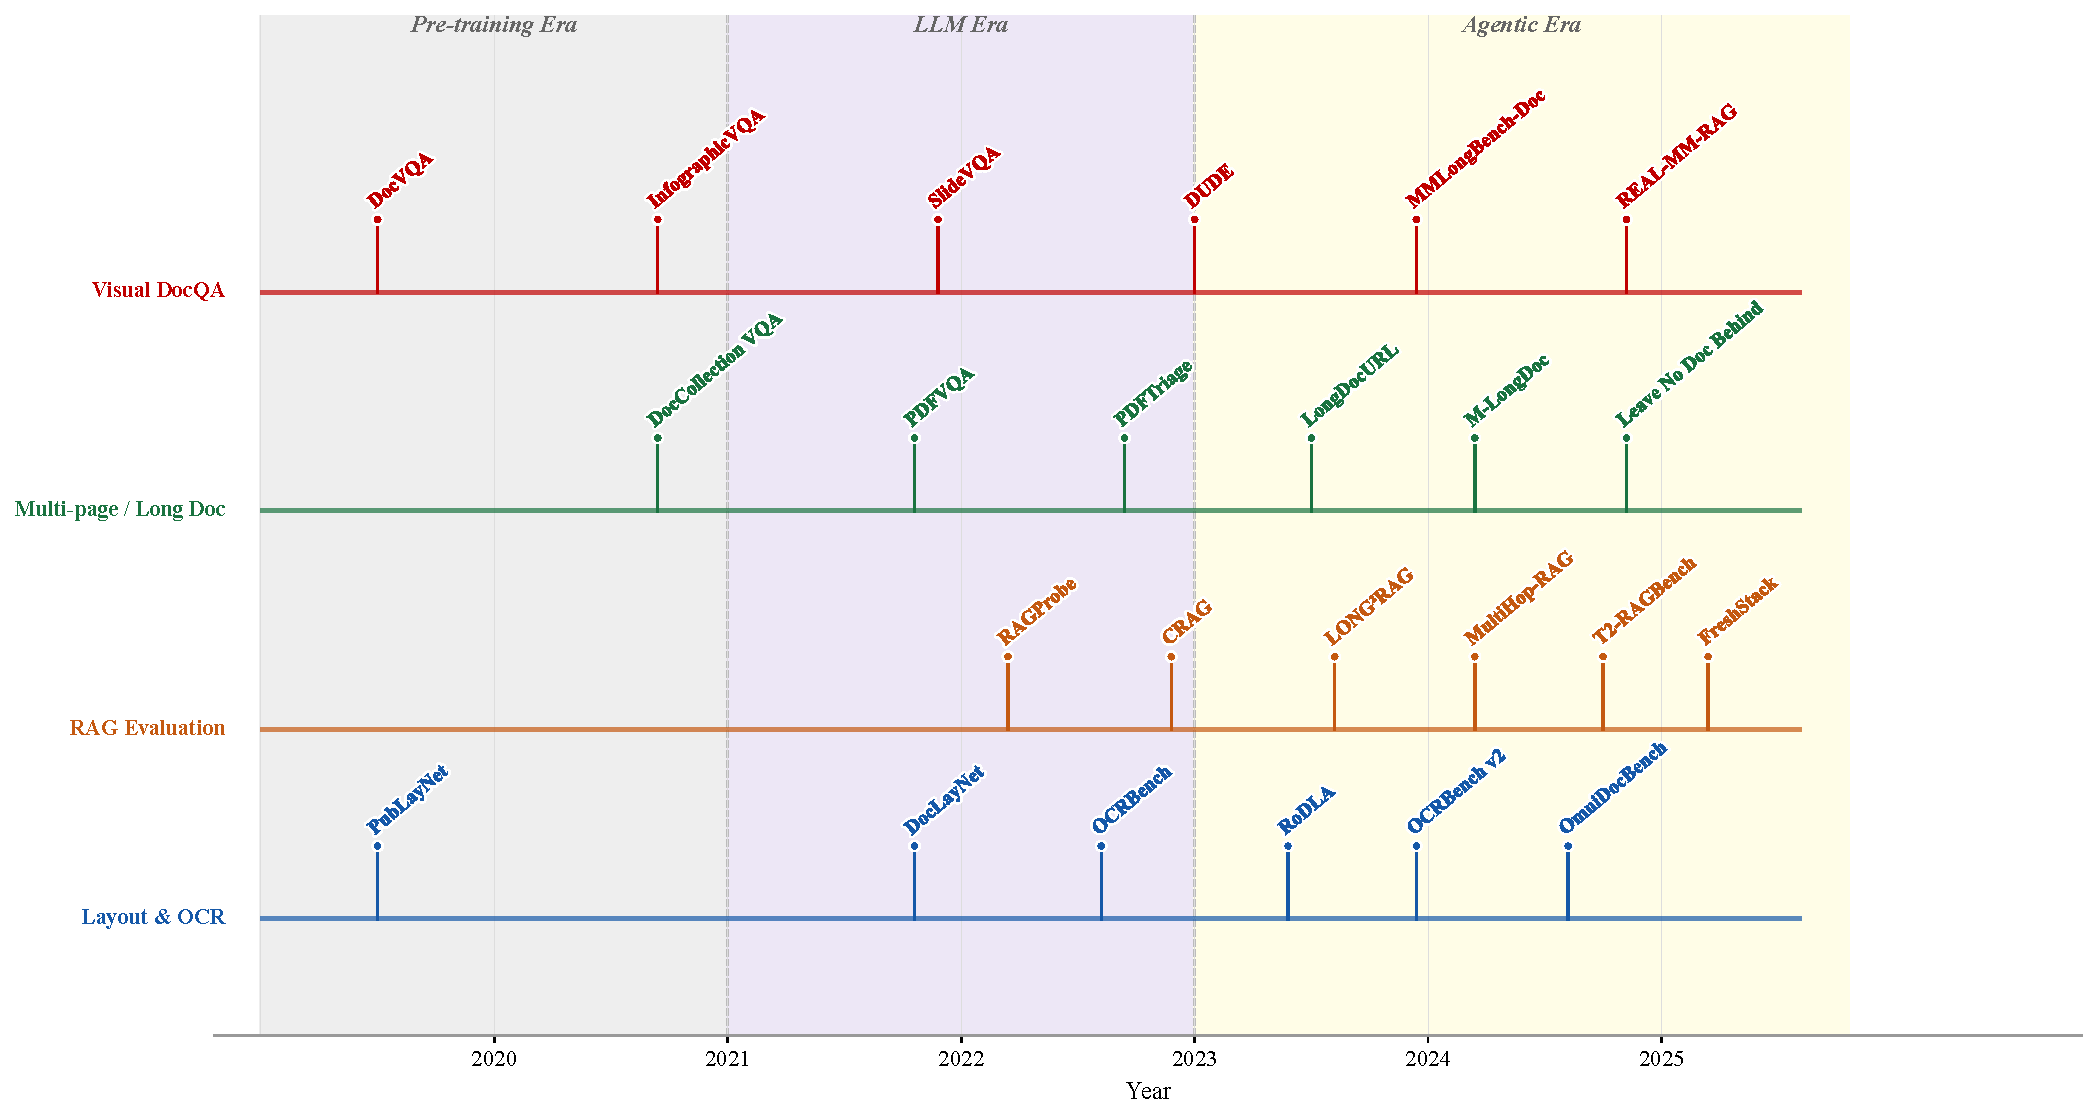
\includegraphics[
    width=0.95\textwidth,
    trim=0cm 0cm 0cm 0cm,
    clip
]{figs_by_qixingyu/fig10.pdf}
\caption{Benchmark landscape for document intelligence (2019--2025): evaluation datasets are organized into four categories---visual document question answering, multi-page and long-document understanding, retrieval-augmented generation evaluation, and layout analysis with optical character recognition---arranged chronologically by year of publication.}
\label{fig:benchmarks}
\end{figure*}

\subsubsection{Document QA Evaluation}

The exploration of document evaluation truly oriented toward RAG appeared in the following stages. RAGProbe \cite{ragprobe2023} is a dataset for evaluating Retrieval-Augmented Generation, covering complex question forms in real products (multiple sub-questions, cross-document, unanswerable, etc.).

Next, a large body of work began to explicitly distinguish the four stages of retrieval / grounding / reasoning / generation and constructed explainable or controllable evaluation frameworks. General and systematic method evaluation benchmarks include the following works. CRAG \cite{crag2024} proposed designing a task set covering multiple domains, document structures, and question types, allowing researchers and engineers to compare different RAG architectures, retrievers, re-rankers, and generative models using the same data and metrics. Such a unified evaluation design allows RAG optimization to move from "subjective parameter tuning" to more quantifiable and reproducible experimental comparisons. Unanswerability Evaluation for RAG \cite{unanswerablerag2024} measures whether a system can correctly refuse to answer when encountering unanswerable queries in documents, systematically expanding "unanswerability" into fine-grained categories for the first time. LONG²RAG \cite{long2rag2024} is an evaluation benchmark for long-context, long-form RAG systems, used to systematically measure the real capabilities of large models in "reading long text, retrieving multiple documents, and generating long answers" scenarios. Fact, Fetch, and Reason \cite{factfetchreason2024} argued for measuring the overall performance of end-to-end systems in real application scenarios. Each sample is a multi-hop QA question where answers are often scattered across multiple Wikipedia articles, sometimes requiring numerical calculation (e.g., "how many times faster"), table queries, temporal reasoning, combining multiple conditions, or post-processing retrieval results.

Many datasets in Chinese and domain-specific directions have also emerged. CRUD-RAG \cite{crudrag2024} is a large-scale Chinese benchmark for RAG systems, abstracting four major application types from the classic CRUD operations of "user interaction with knowledge bases" to perform comprehensive end-to-end and component-level evaluation of RAG. LegalBench-RAG \cite{legalbenchragr2024} is an evaluation benchmark specifically for the "retrieval stage" in the legal domain, used to measure the precision retrieval capabilities of various retrievers on complex legal documents. OmniEval \cite{omnieval2024} is a comprehensive evaluation benchmark for financial RAG systems, used to automatically and comprehensively assess the retrieval and generation capabilities of financial RAG/Agent systems in real financial scenarios. RAGCare-QA \cite{ragcareqa2025}, carefully curated and human-annotated, is a medical RAG evaluation benchmark dataset for systematically evaluating RAG pipelines and model performance in "theoretical medical knowledge QA" scenarios. RAGPPI \cite{ragppi2024} is a RAG benchmark and evaluation framework for the Protein-Protein Interaction (PPI) field, used to evaluate the capability of large models to answer questions related to the biological impact of PPI in drug target discovery scenarios.

Simultaneously, document and multi-modal long-context benchmarks matured rapidly. M3DocVQA \cite{m3docvqa2024} is an open-domain, multi-page, multi-document DocVQA benchmark dataset, primarily serving DocVQA/RAG research for multimodal retrieval and large models. MMLongBench-Doc \cite{mmlongbenchdoc2024} is a benchmark dataset and evaluation framework for multimodal long-context document understanding, mainly used to test the reading comprehension, retrieval, and reasoning capabilities of LVLMs in real long-document PDF scenarios. MMDocBench \cite{mmdocbench2024} is similarly a benchmark and framework for multimodal long-context understanding to test LVLMs in real PDF scenarios. DOCBENCH \cite{docbench2024} is an evaluation benchmark for LLM document reading systems, used to systematically assess the end-to-end capabilities of document reading systems in real interaction scenarios involving "uploading raw documents + asking questions about them." LongDocURL \cite{longdocurl2024} is a large-scale evaluation dataset for long-form multimodal document understanding, used to systematically evaluate the capabilities of multimodal large models in long document understanding, numerical reasoning, and cross-element localization. It focuses on complex PDF documents of dozens or even hundreds of pages, dividing tasks into three main categories: Understanding (U), Reasoning (R), and Locating (L). M-Longdoc \cite{mlongdoc2024} is an evaluation benchmark and framework for "multimodal ultra-long document understanding," used to systematically evaluate and improve the QA and reasoning capabilities of LVLMs/LMMs on hundreds of pages of documents. Proposed in 2024, it focuses on ultra-long PDF documents in realistic scenarios, emphasizing open-ended answering and retrieval augmentation. Leave No Document Behind \cite{leavenodocumentbehind2024} proposed a long-context LLM evaluation benchmark to systematically test models' long-context understanding in "extended multi-document QA" scenarios, defining four types of tasks: Spotlight Locating, Comparison, Clustering, and Chain of Reasoning.

\subsubsection{Real-World Image-Text Interaction Document Evaluation}

As research progresses toward real-world settings, most recent datasets involve image-text interaction. REAL-MM-RAG \cite{realmmrag2025} focuses on real enterprise/document scenarios, emphasizing "difficult retrieval and high robustness" across multiple modalities such as text, tables, and images. CRAG-MM \cite{cragmm2024} is a comprehensive RAG evaluation benchmark for multi-modal, multi-person multi-turn dialogue scenarios, mainly focusing on the real application scenario of "wearable devices + visual QA + retrieval augmentation." Visual-RAG \cite{visualrag2025} is a benchmark and evaluation framework for text-to-image RAG, containing numerous visual knowledge-intensive questions and related image candidate sets. Seeing Through the MiRAGE \cite{mirage2025} is an evaluation framework and benchmark for multimodal RAG, specifically designed to measure the factuality and citation quality of models when retrieving, generating, and citing from multimodal sources such as text, images, audio, and video. UNIDOC-BENCH \cite{unidocbench2025} extracts pages from real enterprise-level PDFs, annotating text blocks, tables, and images with evidence links, and then automatically or semi-automatically constructs multimodal QA pairs. Questions cover four typical RAG tasks: factual retrieval, comparison, summarization, and logical reasoning. VisR-Bench \cite{visrbench2025} proposed a multi-lingual long-document visual retrieval benchmark for visual RAG, focusing on the complete workflow of "retrieving the appropriate page from long multi-page documents and then answering." Benchmarking Retrieval-Augmented Multimodal Generation for Document QA \cite{benchmarkmmrag2025} focuses on mixed image-text information in real complex documents (long PDFs, reports, papers, etc.), including text, formulas, charts, tables, infographics, etc., with complex layouts. Each sample consists of a question, a short answer, and an evidence chain with layout positions. Retrieval for multi-hop and complex reasoning is also gradually developing. MultiHop-RAG \cite{multihoprag2024} is a benchmark and evaluation suite for multi-hop RAG, used to systematically evaluate the retrieval and reasoning capabilities of RAG in complex multi-hop QA scenarios. DocHop-QA \cite{dochopqa2025} focuses on real-world "cross-document, multi-structure, multi-step reasoning" complex information retrieval and reasoning scenarios. Automatically constructed from scientific PDF documents, questions often require aggregating evidence across multiple documents, pages, and structural blocks (paragraphs, tables, captions, etc.) to get the answer, rather than direct lookup in a single text segment. FanOutQA \cite{fanoutqa2024} focuses on so-called "fan-out" questions: one question requires simultaneously finding and integrating information across numerous entities and multiple documents. MHTS \cite{mhts2025} proposed systematically controlling reasoning difficulty to construct high-quality, diverse, and adjustable-difficulty multi-hop QA benchmarks for finer evaluation of RAG retrieval and generation.

RAG evaluation based on structured heterogeneous datasets is also receiving increasing attention. RAG over Tables \cite{ragovertables2025} refers to a set of evaluation benchmarks and frameworks proposed around RAG tasks on tabular data, oriented toward multi-table QA and RAG model evaluation on large-scale tabular corpora. T2-RAGBench \cite{t2ragbench2025} is a text-table hybrid RAG evaluation benchmark for the financial domain, used to systematically assess the model's capability in the complete "retrieval followed by numerical reasoning" process. mmRAG \cite{mmrag2025} is a modular benchmark for heterogeneous/multimodal RAG systems, using a unified framework to evaluate the retrieval and generation capabilities of systems across multiple knowledge sources like text, tables, and knowledge graphs. RAG-based QA over Heterogeneous Data and Text \cite{raghetero2024} is a set of research and experimental configurations around the QUASAR system for evaluating RAG QA capabilities on heterogeneous data sources. Dynamic RAG evaluation datasets based on time have also been proposed. DRAGON \cite{dragon2024} is a dynamic RAG evaluation benchmark for news scenarios, mainly focusing on systematically evaluating the retrieval and generation capabilities of RAG on continuously changing news corpora in a Russian environment. FreshStack \cite{freshstack2025} is an evaluation benchmark and construction framework for technical document retrieval/RAG systems, specifically designed to evaluate the real performance of technical document retrieval and technical RAG QA in 2025 and beyond. It automatically constructs datasets from real community QA, focusing on rapidly evolving and easily contaminated technical fields.

Long-context and retrieval-free control evaluations were subsequently proposed. LaRA \cite{lara2025} focuses on evaluating whether LLMs in typical 2025 applications should rely more on ultra-long context input or obtain information through external retrieval. Ko-LongRAG \cite{kolongrag2025} is an evaluation benchmark specifically for Korean long-context RAG. It simulates real long-document retrieval scenarios through a "retrieval-free construction method" to systematically evaluate various large models on Korean long-context RAG tasks. Summary of a Haystack \cite{summaryhaystack2024} is an evaluation benchmark for long-context large models and RAG systems, focusing on testing the system's robust long-text understanding and aggregation capabilities in million-token contexts. Proposed in 2024, it emphasizes "finding and correctly summarizing important content" in complex multi-document scenarios. Are We on the Right Way for Assessing Document RAG? \cite{rightwaydocumentrag2025} is a systematic analysis and benchmark design study on document-level RAG evaluation methods. It focuses on the deficiencies of current document RAG benchmarks and proposes a new evaluation system, Double-Bench, as an alternative.

In addition to benchmarks directly oriented toward RAG, a series of document visual understanding datasets have systematically characterized the complexity of real documents at visual, structural, and linguistic levels in parallel evolution. These benchmarks do not directly evaluate the retrieval or generation performance of RAG but define the upper limit of input difficulty and the perceptual prerequisites that RAG systems must face in real document scenarios. These include RoDLA \cite{rodla2024}, a robustness benchmark for document layout analysis. It systematically evaluates the stability of layout detection/segmentation model performance under real interference conditions, making it an important robustness evaluation benchmark in the current DLA field. U-DIADS-Bib \cite{udiadsbib2024} is a document layout analysis benchmark for ancient manuscripts, focusing on pixel-level semantic layout segmentation to evaluate and drive algorithm development for tasks such as codex layout understanding, OCR preprocessing, and automatic transcription. M6Doc \cite{m6doc2023} is an open dataset for modern document layout analysis, particularly emphasizing real scenarios, multiple formats, multiple languages, and complex layouts, significantly impacting document understanding and OCR preprocessing. MosaicDoc \cite{mosaicdoc2025} is a large-scale Chinese-English bilingual benchmark for visually rich document understanding, collecting images from newspapers and magazines, containing highly heterogeneous visual elements such as illustrations, titles, subtitles, columns, and advertisement blocks. HW-MLVQA \cite{hwmlvqa2025} is a visual QA dataset and benchmark for multilingual handwritten document understanding, used to evaluate and drive the cross-modal and cross-lingual understanding capabilities of models on real handwritten documents. MTVQA \cite{mtvqa2025} is a benchmark for multilingual text-centric visual QA, used to systematically assess the capabilities of multimodal large models in multilingual scene text understanding and QA. All images come from real-world "text-rich scenes," covering over 20 scene types such as posters, signboards, document screenshots, product packaging, and interface screenshots. IconQA \cite{iconqa2024} is a large-scale visual QA dataset for "diagram reasoning," focusing on iconic scenarios such as abstract charts and textbook illustrations rather than natural images. A Comparative Review \cite{vdureview2025} is a survey work that systematically reviews the evolution of visual document understanding from traditional methods to deep learning and then to multimodal Transformers in recent years. It points out that real-world documents such as invoices, receipts, tables, research reports, and questionnaires contain text, layout, and visual elements simultaneously, thus requiring a concentrated, comparative review for visual document understanding. Together, these works constitute the perceptual and structural foundation for document-level and multimodal RAG systems, explaining why RAG performance in real-world documents is often limited by input parsing and evidence structuring capabilities rather than just the retrieval or generation modules themselves.

\begin{figure*}[t]
\centering
\includegraphics[width=0.95\textwidth]{figs_by_qixingyu/fig11.pdf}
\caption{Hierarchical overview of document understanding and question answering: methods are organized into three main branches---table understanding (covering structure recognition, representation learning, and verifiable reasoning), text-based retrieval-augmented generation (from naive retrieval to graph-enhanced and agentic RAG), and vision-language models for document understanding (spanning foundational models, high-resolution architectures, and OCR-free approaches).}
\label{fig:layout_pipeline2}
\end{figure*}
\balance
\section{Future Research Directions}
Although document intelligence has evolved from OCR-centered pipeline approaches to end-to-end systems capable of cross-page, multimodal understanding and retrieval-augmented generation (RAG), achieving stable deployment in real-world scenarios still faces a series of critical challenges. These challenges lie not only in a model's ability to understand complex documents, but also in system-level evidence organization and reasoning mechanisms, and in risk-oriented evaluation paradigms for real-world deployment. Future research can be advanced along the following three levels.

\paragraph{Verifiable and Structure-Aware Document Understanding.}
Current document question answering systems can often produce seemingly plausible answers, yet these answers frequently lack explicit and verifiable evidence. For example, when asked about a key clause in a contract, a system may generate the correct conclusion but fail to indicate on which page or in which table cell the information is located. This phenomenon---``correct answers but opaque evidence''---limits adoption in high-stakes scenarios, because users cannot easily judge whether the model's reasoning process is trustworthy. Therefore, a key research direction is to jointly model evidence localization and answer generation, so that while producing an answer, the model can explicitly identify the supporting document regions and establish a correspondence between the answer and its evidence, making the reasoning process verifiable rather than merely plausible.

Meanwhile, document understanding is shifting from pipeline methods that rely on explicit text extraction (e.g., OCR) to end-to-end vision-language models that operate directly on visual inputs. Such OCR-free methods can avoid information loss caused by recognition errors, but they also introduce new challenges: these models no longer have explicit textual and structural boundaries, and thus must automatically learn the document organization internally, such as the hierarchical relations between headings and body text, row and column alignments in tables, and semantic associations across fields. Without such structure awareness, even if a model can recognize local content, it is difficult to perform consistent and reliable reasoning.

Therefore, future research should develop structure-aware vision-language modeling methods, enabling models not only to ``see'' document content but also to understand how documents are organized, and to perform content recognition, structural inference, and evidence localization within a unified framework. Such capabilities will transform document QA systems from opaque answer-generation tools into reliable analytical assistants that provide verifiable reasoning processes, thereby supporting more trustworthy automated decision-making and human-AI collaboration.

\paragraph{Multimodal RAG and Agentic Systems for Complex Evidence Organization.}
As document understanding tasks extend from single pages to long documents and even collections of multiple documents, the system's challenge is no longer merely to find the page that contains the answer, but to integrate information scattered across different locations into a consistent and reliable conclusion. For instance, an answer may partly come from textual descriptions, partly from tabular data, and partly from figures or supplementary notes on later pages. Although current methods can retrieve relevant content, they often lack effective mechanisms to confirm whether these pieces of information refer to the same entity or are logically consistent, which can lead to incomplete or even contradictory reasoning results. Therefore, future research should develop finer-grained retrieval and representation methods that allow models to localize specific regions in documents, establish cross-page and cross-modal associations, and continuously verify consistency among different evidence during reasoning, rather than relying on one-shot retrieval results.

In addition, in real application scenarios, document understanding is typically not accomplished by a single model, but by the collaboration of multiple functional modules---for example, layout parsing to identify document structure, table parsing to extract structured data, retrieval modules to locate relevant content, and rule-based or computational modules to perform precise verification. Compared with a single model, an agentic system that integrates these tools can dynamically choose appropriate processing steps according to task requirements, thereby improving overall capability. However, this also brings new research challenges, including how to ensure that the model can reliably select and invoke appropriate tools, how to prevent errors from accumulating throughout multi-step processing, and how to explicitly indicate that a reliable conclusion cannot be reached when evidence is insufficient or conflicting, rather than generating a superficially plausible but ungrounded answer. Addressing these issues will enable document understanding systems to evolve from simple information extraction tools into intelligent systems that can integrate complex evidence and provide reliable reasoning processes.

\paragraph{Risk-Oriented Data and Evaluation Paradigms for Real-World Deployment.}
Most existing evaluations of document understanding systems are built on well-structured, high-quality benchmark data, such as well-typeset PDFs or form documents with fixed templates. In such environments, models can often achieve high accuracy. However, documents in real business scenarios are usually more complex: scans may be blurry, skewed, or occluded; documents from different sources can vary substantially in format and language; and key information may be scattered across long contexts or even multiple documents. This gap between training and evaluation environments and real-world conditions leads to models that perform well on benchmarks but exhibit significant performance degradation in practice. Therefore, future evaluations should pay more attention to generalization under real distributions, including robustness to low-quality documents, adaptability to cross-domain documents, and computational efficiency and stability when handling long documents.

Moreover, existing evaluations typically focus only on whether the final answer is correct, but in practical applications an equally important question is whether the answer is grounded in verifiable evidence. For instance, even if a system occasionally produces the correct answer, users may still find it hard to trust the result if the system cannot explain where the evidence comes from. Therefore, future evaluations should move beyond a single accuracy metric to multi-dimensional metrics that reflect system reliability, such as whether evidence is correctly localized, whether the reasoning process is internally consistent, whether the system can explicitly indicate uncertainty when it fails, and whether errors are diagnosable. Such risk-oriented evaluation paradigms will more accurately reflect a system's trustworthiness in real-world conditions, and will shift research goals from merely improving average accuracy to building document intelligence systems whose behavior is predictable, whose reasoning is verifiable, and whose behavior in real-world deployment is reliable.



\bibliography{custom}
\appendix
\clearpage
\end{document}